% -----------------------------------------------------------------------------
% main_v6.tex - revised manuscript for the Tethys CONUS sectoral water demand
% Data Descriptor in Scientific Data (Submission 8d19b29c-d61a-4dbe-b3c4-0e38748a5261).
% -----------------------------------------------------------------------------

\documentclass[fleqn,10pt]{wlscirep}
%\usepackage[utf8]{inputenc}
\usepackage[T1]{fontenc}
\usepackage{textcomp}
\usepackage{lineno}
\usepackage{booktabs}
\usepackage{xurl}

\usepackage{tikz}
\usetikzlibrary{positioning, arrows.meta, fit, backgrounds, shapes.geometric}

\usepackage{graphicx}
\graphicspath{{figures/}}

%\usepackage{biblatex}
%\addbibresource{bib/Tethys.bib} 

\linenumbers

\title{A high-resolution monthly sectoral water demand dataset for the contiguous United States from 1980--2100}

\author[1*]{Cameron Bracken}
\author[2*]{Hassan Niazi}
\author[1]{Travis Thurber}
\author[2]{Isaac Thompson}
\author[1]{Kazi Tamaddun}
\author[3]{Hisham Eldardiry}
\author[1]{Kendall Mongird}
\author[1,3]{Nathalie Voisin}
\author[1]{Ning Sun}
\author[1]{Jennie Rice}

\affil[1]{Pacific Northwest National Laboratory, Richland, WA, USA}
\affil[2]{Joint Global Change Research Institute, Pacific Northwest National Laboratory, College Park, MD, USA}
\affil[3]{University of Washington, Seattle, WA, USA}

\affil[*]{corresponding author(s): Cameron Bracken (cameron.bracken@pnnl.gov), Hassan Niazi (hassan.niazi@pnnl.gov)}

\begin{abstract}
U.S. water demand varies sharply by sector and region as land use, population, weather patterns, and economic activity coevolve. High-resolution water demand data are required to capture these dynamics and to support integrated energy-water-land modeling and local and regional water scarcity assessments. We present a gridded (1/8$^{\circ}$), monthly, multisector water demand dataset for the contiguous United States (CONUS) covering 1980--2100 across one historical period and eight future scenarios spanning a wide but plausible range of atmospheric conditions, emissions constraints, and economic, technological, and population growth assumptions. The dataset covers six demand sectors (irrigation, thermoelectric, municipal covering public supply and self-supplied domestic, livestock, manufacturing, and mining) and 25 underlying subsectors, separately for withdrawals and consumption, and attributes water use to groundwater or surface water sources for each grid cell. The historical record is validated over 2010--2019 against the United States Geological Survey (USGS) water use reanalysis for the three largest sectors at the Hydrologic Unit Code 6 (HUC6) scale, with Pearson correlations from 0.72 to 0.95. The dataset advances prior global products through state-level sectoral demands, future power plant siting projections, consistent meteorological, population, and land use forcing across scenarios, and a spatial resolution refinement from 1/2$^{\circ}$ to 1/8$^{\circ}$ (approximately 10--14~km at CONUS midlatitudes).
\end{abstract}
\begin{document}

\flushbottom
\maketitle
% Click the title above to edit the author information and abstract

\thispagestyle{empty}

% -----------------------------------------------------------------------------
\begin{figure}[!ht]
\centering
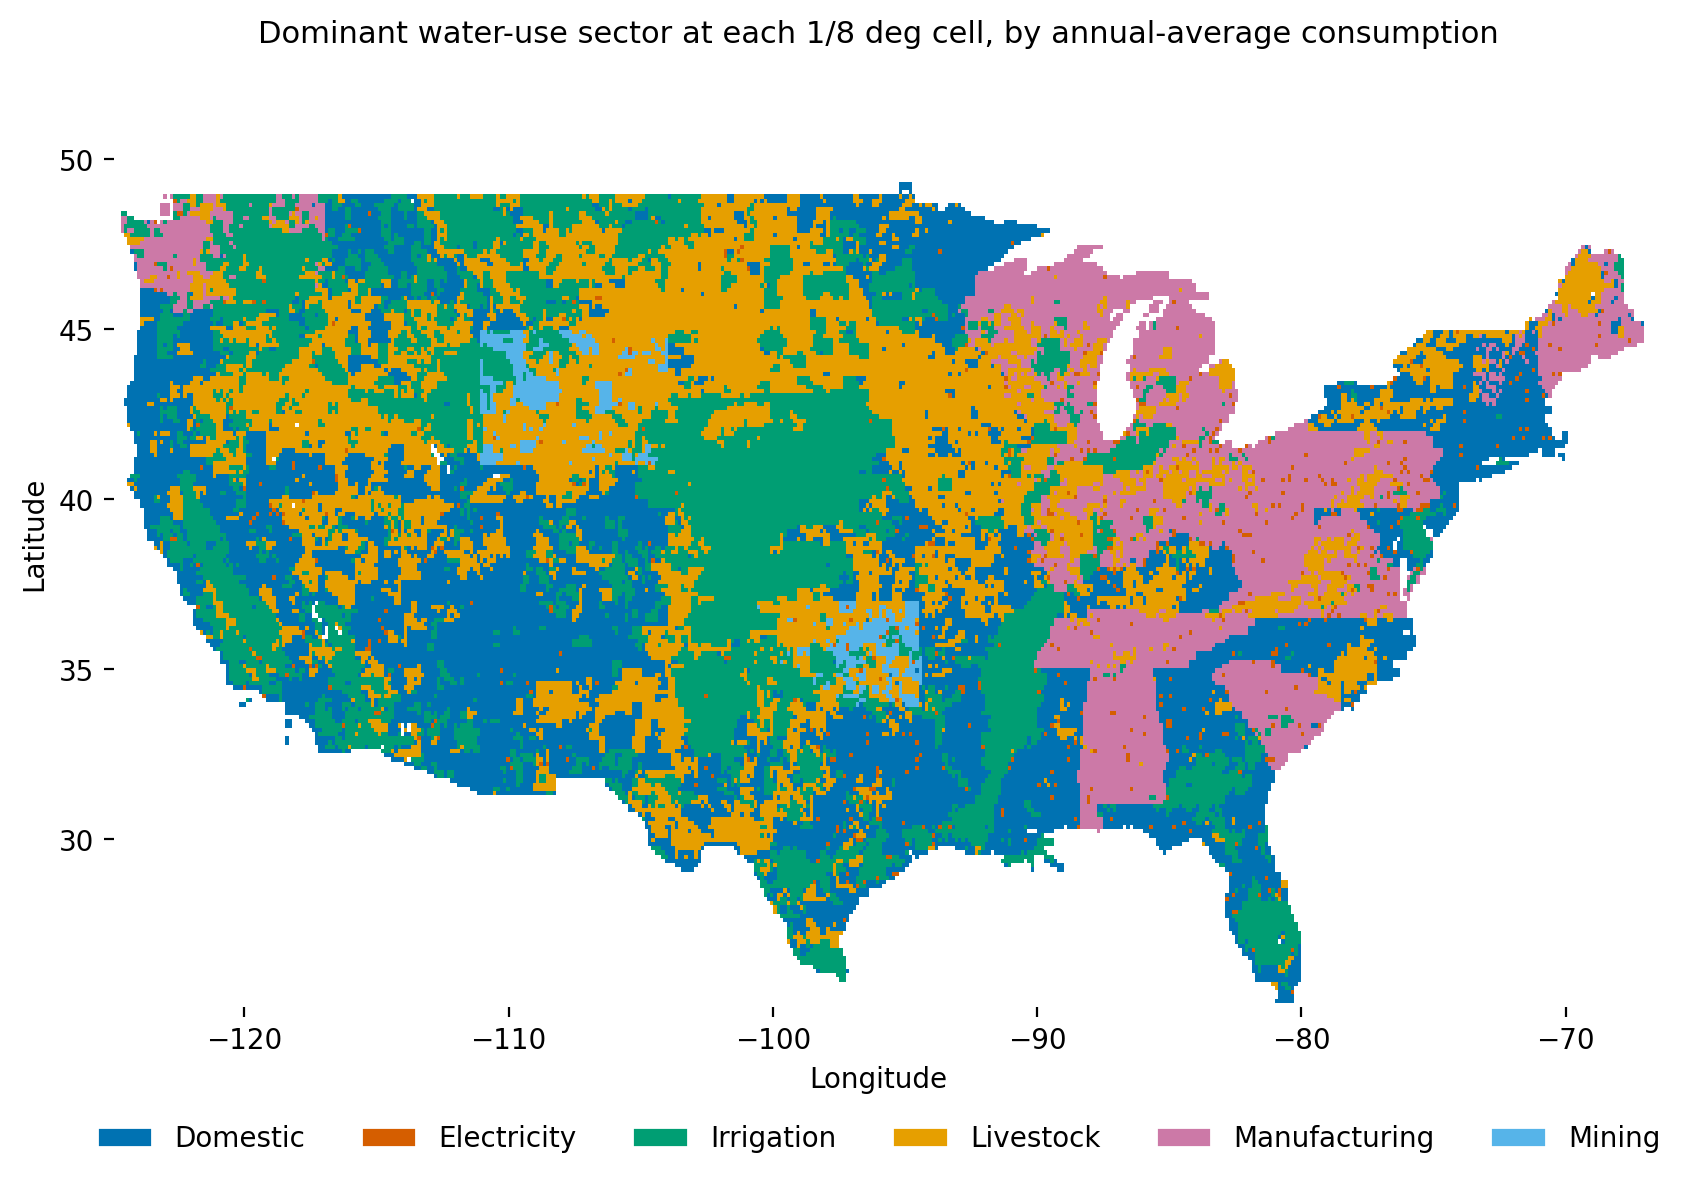
\includegraphics[width=\linewidth]{usage1-dominant-sector-tethys-grid.png}
\caption{Dominant water use sector at each 1/8$^{\circ}$ cell across CONUS, by mean annual consumption in the historical Tethys dataset\cite{bracken2026TethysDataSet} (1980--2019), overlaid with U.S.\ state boundaries. Spatial patterns reflect the multisector and heterogeneous nature of U.S.\ water demand, including irrigation across the High Plains, Mississippi Embayment, Snake River Plain, and California Central Valley, livestock across western rangelands, thermoelectric demand at power generation sites, municipal (\texttt{Domestic}) demand surrounding metropolitan areas, and manufacturing and mining adding regional structure.}
\label{fig:dominant-sector}
\end{figure}

\section*{Background \& Summary}

Humans depend on water for irrigation, thermoelectric cooling, municipal, manufacturing (equivalent to industrial manufacturing, and referred to as manufacturing throughout), mining, and livestock purposes. The relative contribution of these sectors varies sharply across regions and over time. Global water demand is projected to rise through the 21st century under combined socioeconomic pressures and evolving meteorological patterns\cite{WWDR2019, Niazi2024PeakWater, Awais2024Preprint}. Demand-side drivers, not supply-side limits, dominate most projected shifts in water scarcity\cite{Graham_2020, Awais2024Preprint, Kyle2023Sustainability}. Even where regional supply appears ample, scarcity can manifest locally when demand and availability are mismatched in space or time\cite{HADJIMICHAEL23}. Modeling water scarcity under complex and dynamic future conditions requires demands resolved at the spatial and temporal scales relevant to management decisions.

High-resolution multisector water demand projections remain scarce, constraining integrated modeling of energy-water-land systems and local and regional water scarcity. Reconstructed historical datasets, such as Huang et al.\ (2018)\cite{Huang2018}, provide gridded benchmarks for past decades but do not extend to future scenarios. Historical U.S.\ water use records are also challenging to harmonize at watershed scales because state reporting requirements and measurement practices vary widely, compiled totals often follow county or state boundaries rather than hydrologic units, and withdrawals recorded at points of diversion (including interbasin transfers) can differ from locations of use\cite{naseri2025united,Luukkonen2025JAWRA}. Projecting water demand into the future requires an integrated model that links global energy, land, and water systems, yet its outputs typically lack the spatial detail required for river routing or local management modeling\cite{Wada_2017, van_Vliet_2021}. While aggregate U.S.\ water demands at coarse resolutions are generally consistent in the literature\cite{Zhao_gcamusa_water, naseri2025united, Stets2025USGS}, translating them to finer scales requires spatial and temporal downscaling\cite{hess-17-4555-2013, van_Vliet_2021, Jones_2024}. The fidelity of downscaling depends strongly on the choice of proxy variables and the consistency of driving scenarios. Khan et al.\ (2023)\cite{Khan2023} produced the first global multisector water demand product with Tethys at 1/2$^{\circ}$ monthly resolution, yet resolving national management decisions and local impacts across CONUS requires finer spatial resolution and internally consistent scenario forcings of meteorology, land use, and population.

We present such a dataset with multisector coverage across multiple scenarios, refined to 1/8$^{\circ}$ monthly resolution across CONUS (Table~\ref{tab:prior-datasets}). The published record contains gridded monthly water withdrawals and consumption for six sectors (irrigation, thermoelectric, municipal covering public supply and self-supplied domestic, livestock, manufacturing, and mining) aggregating 25 underlying subsectors from the Global Change Analysis Model with subnational detail for the U.S.\ (GCAM-USA\cite{Calvin2019GCAM,Binsted_2022,Zhao_gcamusa_water,Zhao2024}): 11 crop and land use types, 7 thermoelectric generation types, 5 livestock species, plus municipal, manufacturing, and mining. Dataset extent covers CONUS for the historical period (1980--2019) and eight future scenarios (2020--2100) sampling future atmospheric and socioeconomic conditions, along with groundwater and surface water source shares for each grid cell.

Compared with the prior global Tethys product\cite{Khan2023}, this dataset advances U.S.\ water demand representation in six ways. First, spatial resolution is refined from 1/2$^{\circ}$ to 1/8$^{\circ}$ (a $16\times$ increase in grid cell density), capturing finer HUC-level demand variation relevant to river routing, reservoir operations, and regional planning. Second, whereas Khan et al.\cite{Khan2023} disaggregated a single national U.S.\ total from global GCAM, this dataset uses GCAM-USA\cite{Zhao_gcamusa_water,Zhao2024,Calvin2019GCAM,Binsted_2022}, which resolves electricity, manufacturing, mining, and municipal (\texttt{Domestic}) demands by state and crop irrigation demands at state and basin intersections, preserving state sectoral demands and regulatory differences. Third, in place of population centroids as a proxy for retail electricity load\cite{Khan2023}, thermoelectric water demand is sited at power generation facilities using Capacity Expansion Regional Feasibility (CERF)\cite{Vernon2021,Mongird2025CERF} projections at $\approx$1~km resolution (and 2015 Global Power Plant Database v1.3 locations\cite{globalpowerplantdb} historically). Fourth, in place of a static base year population map\cite{Khan2023}, municipal, manufacturing, and mining demands use Shared Socioeconomic Pathway (SSP) gridded population projections\cite{Jones_2016,Jones2020SEDAC} harmonized with state SSP trajectories\cite{Zoraghein2020Zenodo}, capturing demographic divergence between SSP3 and SSP5. Fifth, monthly irrigation weights combine water deficit with a growing season index (GSI) rather than a seasonal profile based only on temperature\cite{Khan2023}. Sixth, while prior U.S.\ studies have delineated groundwater and surface water use for historical benchmark periods\cite{Marston2018WRR,Dieter2018USGS,Stets2025USGS}, the prior Tethys product\cite{Khan2023} lacked water source attribution. Here we extend groundwater and surface water source shares for each grid cell across scenario projections through 2100 by anchoring GCAM-USA basin trajectories to the USGS HUC12 reanalysis\cite{Stets2025USGS}.

Figure~\ref{fig:dominant-sector} shows the dominant consumptive demand sector at each 1/8$^{\circ}$ cell across CONUS. In the western and central U.S., spatial patterns follow the distribution of cropland, rangeland, and resource proxies across state borders. In several eastern states (such as along the Alabama--Mississippi and Tennessee--Georgia borders), transitions between manufacturing and municipal (\texttt{Domestic}) dominance align with state boundaries. This pattern arises from the downscaling structure, which uses GCAM-USA as its input. Municipal, manufacturing, and mining demands are resolved at the state level, which can result in discontinuities at state boundaries (see Limitations for details). Overall, the dataset supports hydrologic, energy-water-land, and integrated multisector dynamics modeling, including assessments of bulk power system resilience, regional water scarcity, and conjunctive groundwater and surface water management across scenarios.


\begin{table}[!ht]
\centering
\small
\begin{tabular}{lllll}
\toprule
\textbf{Dataset} & \textbf{Spatial res.} & \textbf{Temporal res.} & \textbf{Scenarios} & \textbf{Sectors} \\
\midrule
Huang et al.\cite{Huang2018}                   & 0.5$^{\circ}$ global & monthly & historical (1971--2010) & 6 sectors \\
Khan et al.\cite{Khan2023}                     & 0.5$^{\circ}$ global & monthly & historical + SSP/RCP futures & 6 sectors \\
Medalie et al.\cite{Stets2025USGS,Haynes2023USGS,Luukkonen2023USGS,Galanter2023USGS} & HUC12 CONUS & monthly & historical (2010--2020) & 3 sectors \\
Naseri \& Marston\cite{naseri2025united}       & facility or user, & annual & historical & multisector  \\
                                               & 42 U.S. states & (varies by state) &  &   \\
van Vliet et al.\cite{van_Vliet_2021}          & country/basin & annual & historical + SSP & 6 sectors \\
Wada et al.\cite{Wada_2017}                    & 0.5$^{\circ}$ global & monthly & historical + projections & 4 sectors \\
\textbf{This work}                             & \textbf{0.125$^{\circ}$ CONUS} & \textbf{monthly} & \textbf{hist.\ + 2 RCPs $\times$ 2 GCMs $\times$ 2 SSPs} & \textbf{6 sectors} \\
                                               &                                &                  & \textbf{(8 future scenarios)}                                & \textbf{(25 subsectors)} \\
                                               &                                &                  &                                                              & \textbf{+ gw/sw source share} \\
\bottomrule
\end{tabular}
\caption{Gridded multisector water demand datasets that overlap in scope with the dataset presented here. The current dataset increases spatial resolution by a factor of four (16$\times$ the number of grid cells) over its immediate Tethys predecessor\cite{Khan2023}, adds groundwater and surface water source shares for every grid cell, and uses internally consistent scenarios of population, land use, and meteorological forcing. The six sectors aggregate 25 underlying GCAM-USA subsectors: 11 crop and land use types (irrigation), 7 thermoelectric generation types (electricity), 5 livestock species, plus municipal, manufacturing, and mining. Abbreviations: res., resolution; CONUS, contiguous United States; HUC12, 12-digit Hydrologic Unit Code; hist., historical (1980--2019); RCPs, Representative Concentration Pathways; GCMs, General Circulation Models; SSPs, Shared Socioeconomic Pathways; gw/sw, groundwater and surface water.}
\label{tab:prior-datasets}
\end{table}

% -----------------------------------------------------------------------------
\section*{Methods}
We produce the dataset by applying Tethys\cite{niazi_2026_20552731} (\href{https://github.com/JGCRI/tethys}{github.com/JGCRI/tethys}), a mass-conserving spatiotemporal downscaling framework, to GCAM-USA outputs\cite{Zhao2024} (\href{https://doi.org/10.57931/2428940}{doi.org/10.57931/2428940}) together with sectoral spatial proxies and monthly temporal downscaling weights derived from meteorology. Workflow scripts and configurations are maintained in the integration metarepository\cite{cambrackenIMMMSFATethys_integration_metarepoV1012026} (\href{https://github.com/IMMM-SFA/tethys_integration_metarepo}{github.com/IMMM-SFA/tethys\_integration\_metarepo}; archived on Zenodo at \href{https://doi.org/10.5281/zenodo.20600510}{doi.org/\allowbreak 10.5281/\allowbreak zenodo.20600510}), and preprocessed model inputs and region masks used to execute the workflow are archived in the companion input dataset on MSD-Live\cite{brackenDataTethys_integration_metarepo} (\href{https://doi.org/10.57931/3366010}{doi.org/10.57931/3366010}). GCAM-USA computes water withdrawals and water consumption separately prior to Tethys downscaling using water intensity coefficients by sector, fuel, and technology\cite{Calvin2019GCAM,Binsted_2022}. Tethys then downscales withdrawals and consumption in separate runs using identical spatial proxies and monthly temporal weights. The result is a 1/8$^{\circ}$ monthly water demand record for 6 sectors and 25 GCAM-USA subsectors, for one historical period (1980--2019) and eight future scenarios (2020--2100). The Tethys downscaling chain (Figure~\ref{fig:schematic}) converts state and basin water demand outputs from GCAM-USA\cite{Zhao_gcamusa_water,Zhao2024,Calvin2019GCAM,Binsted_2022} into 1/8$^{\circ}$ monthly gridded fields by applying sectoral spatial proxies from Demeter land use\cite{Vernon-2018} (\href{https://github.com/IMMM-SFA/demeter}{github.com/IMMM-SFA/demeter}), CERF power plant siting\cite{Vernon2021,Mongird2025CERF} (\href{https://github.com/IMMM-SFA/cerf}{github.com/IMMM-SFA/cerf}) and historical Global Power Plant Database (GPPD) v1.3 records\cite{globalpowerplantdb} (\href{https://datasets.wri.org/dataset/globalpowerplantdatabase}{datasets.wri.org/dataset/globalpowerplantdatabase}), SSP population projections\cite{Jones_2016,Jones2020SEDAC,Zoraghein2020Zenodo}, and Gridded Livestock of the World v3 (GLW~3)\cite{Gilbert2018} (\href{https://dataverse.harvard.edu/dataverse/glw_3}{dataverse.harvard.edu/dataverse/glw\_3}), and distributing annual values into months using meteorological indicators derived from the Thermodynamic Global Warming (TGW)\cite{Jones2023TGW} (\href{https://tgw-data.msdlive.org/}{tgw-data.msdlive.org}) dataset (deficit, growing season index, and heating and cooling degree days). A postprocessing step assigns each cell's groundwater and surface water source share by anchoring basin GCAM-USA trajectories to the USGS HUC12 reanalysis baseline\cite{Stets2025USGS,Haynes2023USGS,Luukkonen2023USGS}. The downscaling process is executed for the historical period and each of the eight future scenarios.

The remainder of this section is organized in two parts. The first part describes the exogenous scenarios and inputs to Tethys: GCAM-USA state and basin water demands, the TGW meteorological forcing, the Demeter land use projections, and the CERF power plant projections. The second part describes the Tethys mechanics: spatial downscaling (Eq.~\ref{eq:spatial}) with sectoral proxies, temporal downscaling with sectoral monthly weights, and groundwater and surface water source share postprocessing (Eq.~\ref{eq:source-shares}). The closing subsection documents the modular one-way coupling design.

\begin{figure}[!ht]
\centering
% Workflow figure is built natively in TikZ and compiled separately as a
% standalone PDF. Source: flow-chart.tex; rebuild with `lualatex flow-chart.tex`.
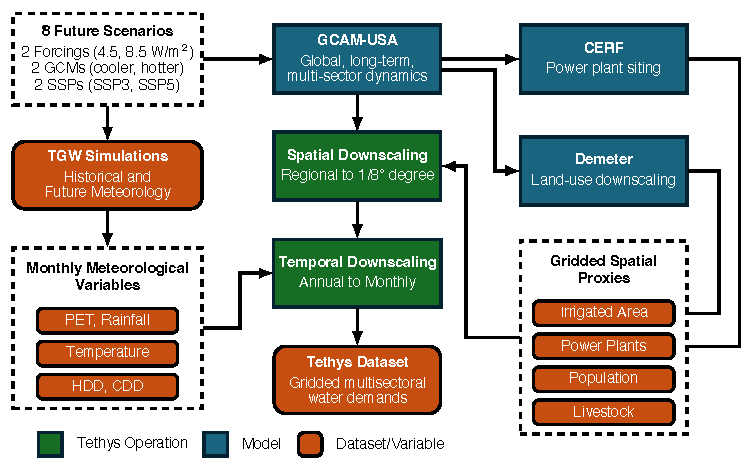
\includegraphics[width=0.9\textwidth]{figures/flow-chart.pdf}
\caption{Workflow for producing the Tethys CONUS multisector water demand dataset across the historical period (1980--2019) and eight future scenarios (2020--2100; Table~\ref{tab:scenarios}). The eight future scenarios combine two Representative Concentration Pathway (RCP) radiative forcing levels (4.5 and 8.5~W/m$^2$), two General Circulation Model (GCM) temperature sensitivity groups (hotter and cooler), and two Shared Socioeconomic Pathways (SSP3 and SSP5). For both the historical run and each future scenario, Tethys (green boxes) performs two downscaling operations: spatial downscaling of 5-year regional demands to the 1/8$^{\circ}$ CONUS grid, followed by linear interpolation from 5-year steps to annual values and temporal downscaling of annual demands to monthly resolution. Spatial downscaling uses gridded proxies derived from Demeter\cite{Vernon-2018} (land use), CERF\cite{Vernon2021,Mongird2025CERF} (projected power plant siting, with 2015 GPPD v1.3\cite{globalpowerplantdb} substituted in the historical period), Jones and O'Neill\cite{Jones_2016,Jones2020SEDAC} and Zoraghein and O'Neill\cite{Zoraghein2020Zenodo} (SSP population), and GLW~3\cite{Gilbert2018} (livestock). Temporal downscaling uses monthly meteorological variables derived from the Thermodynamic Global Warming (TGW) dataset\cite{Jones2023TGW} (historical baseline driven by ERA5 and thermodynamically perturbed future runs), including potential evapotranspiration (PET), precipitation, mean temperature, heating degree days (HDD), cooling degree days (CDD), and growing season index (GSI).} 
\label{fig:schematic}
\end{figure}

\subsection*{GCAM-USA state/basin-level water demand}

% COMMENT-ning: "policy" is off-limits 
% COMMENT-ning: you really mean livestock demands are provided at two different spatial resolutions? or there are different spatial resolutions for the U.S. and the rest of the world in GCAM? If so, i think we only need to report the resolution for the U.S., given the CONUS focus of this paper?
Regional water demand inputs come from GCAM-USA (IM3 Phase~2 official simulations\cite{Zhao2024}, publicly archived at \href{https://doi.org/10.57931/2428940}{doi.org/\allowbreak 10.57931/\allowbreak 2428940})\cite{Zhao_gcamusa_water,Calvin2019GCAM,Binsted_2022}. GCAM is a market equilibrium integrated assessment model that allocates supply and demand across coupled energy, water, land, and economic sectors under scenario assumptions on population, productivity, and technological development. GCAM-USA resolves U.S.\ electricity generation, manufacturing, mining, and municipal demands at the state level, livestock demands at the national/regional level, and crop irrigation demands at state and basin intersections, at 5-year intervals. Within Tethys, 5-year regional demands are first spatially downscaled to the 1/8$^{\circ}$ grid and then linearly interpolated to annual values before monthly temporal downscaling is applied. Separate GCAM-USA runs drive the historical baseline and each of the eight future scenarios. We refer readers to Mongird et al.\cite{Mongird2025CERF}, Zhao et al.\cite{Zhao_gcamusa_water}, and Binsted et al.\cite{Binsted_2022} for the full energy-water-land coupling description of GCAM-USA and limit our scope here to how GCAM-USA outputs feed the Tethys workflow shown in Figure~\ref{fig:schematic}.

% COMMENT-ning: i removed the word "policy"
The dataset's historical period spans 1980--2019 and future scenarios span 2020--2100 across eight scenarios\cite{Zhao_gcamusa_water,Zhao2024,Mongird2025CERF}. The future scenarios sample three dimensions: radiative forcing target (\texttt{rcp45} representing moderate emissions constraints and moderately hotter conditions, versus \texttt{rcp85} representing unmitigated emissions and severely hotter conditions), GCM temperature sensitivity over CONUS (cooler versus hotter CMIP6 model groups), and socioeconomic narrative\cite{ONeill2017SSP}. Following O'Neill et al.\cite{ONeill2017SSP}, SSP3 (\textit{Regional Rivalry}) represents a world of reduced global integration, slower economic development and technological change, and declining U.S.\ population. In contrast, SSP5 (\textit{Fossil-Fueled Development}) represents rapid globalized economic growth, lifestyles intensive in energy and resources, rapid technological progress, and substantial U.S.\ population growth driven largely by higher net immigration. We retain the prefix ``rcp'' in scenario directory names for consistency with upstream IM3 datasets, although the underlying thermodynamic perturbation simulations are derived from CMIP6 rather than CMIP5\cite{Jones2023TGW,Mongird2025CERF}. The historical and eight future scenario directory names (for example, \texttt{rcp45cooler\_ssp3}) appear in Table~\ref{tab:scenarios}, and CONUS demand behavior across scenarios is shown in Figure~\ref{fig:scenarios}.

\subsection*{Meteorological forcing (TGW)}

Historical and projected meteorological data come from the TGW dataset \cite{Jones2023TGW} (\href{https://tgw-data.msdlive.org/}{tgw-data.msdlive.org}), which provide hourly atmospheric variables at 12~km resolution over CONUS, dynamically downscaled with the Weather Research and Forecasting (WRF) model from a 30~km ERA5 historical baseline (1980--2019) and from monthly thermodynamic perturbations derived from CMIP6 (2020--2100). The thermodynamic perturbation approach replays historical weather sequences with added thermodynamic signals, retaining the synoptic structure of observed weather while shifting its mean state and humidity and temperature relationships to match each future scenario. For each simulation we compute daily potential evapotranspiration (PET), precipitation ($P$), mean temperature, heating degree days (HDD), cooling degree days (CDD), and a growing season index (GSI). These variables are aggregated to monthly totals or means, reprojected to the Tethys 1/8$^{\circ}$ CONUS grid, and archived in the companion input dataset\cite{brackenDataTethys_integration_metarepo}.

The monthly water deficit used in irrigation temporal downscaling is $\Delta_m = \max\!\big(\text{PET}_m - P_m,\, 0\big)$ (with small residual weighting when $P_m > \text{PET}_m$ following Moore et al.\cite{Moore_2015}). The monthly GSI is derived from a simplified version of Jolly et al.\cite{Jolly_2005}, retaining the daily minimum temperature ($iT_{\min}$) and daylength photoperiod indicators ($iPhoto$) while omitting the vapor pressure deficit term. For each day $d$,
\begin{equation}
iT_{\min,d}(T_{\min,d}) = \min\!\left(\max\!\left(\frac{T_{\min,d}+2}{7},\,0\right),\,1\right), \qquad
iPhoto_d(L_d) = \min\!\left(\max\!\left(L_d - 10,\,0\right),\,1\right),
\label{eq:gsi-components}
\end{equation}
where $T_{\min,d}$ is the daily minimum air temperature (\textdegree C) and $L_d$ is the daylength (hours). Monthly GSI is the mean daily product over the month $m$,
\begin{equation}
GSI_m = \big\langle iT_{\min,d} \cdot iPhoto_d \big\rangle_{d \in m}.
\label{eq:gsi-monthly}
\end{equation}
Preprocessing code is archived in the integration metarepository\cite{cambrackenIMMMSFATethys_integration_metarepoV1012026} (see Code availability).

\subsection*{Downscaled land use projections (Demeter)}

Irrigated crop area maps at 1/8$^{\circ}$ come from Demeter\cite{Vernon-2018} (\href{https://github.com/IMMM-SFA/demeter}{github.com/IMMM-SFA/demeter}), a land use spatial disaggregation model that reconciles a high-resolution land use baseline with GCAM-USA's regional land use and land cover change (LULCC) projections. Demeter uses transition priority rules that distinguish intensification (increase of a land type within a cell) from extensification (spread from an adjacent cell). For irrigation, Demeter outputs cover the crop classes reported by GCAM-USA (Corn, Wheat, Rice, RootTuber, OilCrop, SugarCrop, OtherGrain, FiberCrop, FodderGrass, FodderHerb, biomass, MiscCrop, and PalmFruit, aggregated with other arable land into 11 irrigated subsectors in Tethys) and are archived in the companion input dataset\cite{brackenDataTethys_integration_metarepo}. The crop-specific irrigated area fields serve as the spatial proxy for irrigation in Tethys spatial downscaling.

\subsection*{Power plant siting projections (CERF)\label{sec:cerf}}

% COMMENT-kendall: Can we also cite the Sci Data CERF paper? https://www.nature.com/articles/s41597-023-02694-y
The Capacity Expansion Regional Feasibility (CERF) model\cite{Vernon2021,Mongird2025CERF} (\href{https://github.com/IMMM-SFA/cerf}{github.com/IMMM-SFA/cerf}) sites future thermoelectric and non-thermoelectric capacity at 1~km resolution based on siting feasibility (exclusion layers, cooling water access) and locational economics, conditional on the GCAM-USA state capacity trajectory for each scenario. The sited thermoelectric facilities represent seven fuel categories (coal, natural gas, refined liquids/oil, nuclear, biomass, geothermal, and concentrated solar thermal). Plants sited by CERF are aggregated to 1/8$^{\circ}$ grid cells, and grid cell installed capacity in megawatts (MW) serves as the spatial proxy for thermoelectric demand. For the historical period (1980--2019), we use a 2015 plant inventory derived from the Global Power Plant Database v1.3 (GPPD)\cite{globalpowerplantdb} (\href{https://datasets.wri.org/dataset/globalpowerplantdatabase}{datasets.wri.org/dataset/globalpowerplantdatabase}) harmonized with IM3 historical plant attributes in place of CERF projections (preprocessing scripts in the integration metarepository\cite{cambrackenIMMMSFATethys_integration_metarepoV1012026} and gridded capacity inputs in the companion input dataset\cite{brackenDataTethys_integration_metarepo}). Plant U.S.\ Energy Information Administration (EIA) water withdrawal and consumption reports are not ingested directly by Tethys, although EIA generator capacities inform GPPD v1.3 and EIA cooling water records inform the USGS thermoelectric reanalysis\cite{Galanter2023USGS,Harris2025,skinnerWaterWithdrawalConsumption2025} used for validation. While upstream GCAM-USA\cite{Binsted_2022} and CERF\cite{Mongird2025CERF} differentiate plant cooling technologies (once-through, recirculating, cooling pond, and dry cooling) when computing state water demands and siting feasibility, Tethys spatial proxy preprocessing sums plant capacity into the seven fuel subsectors without splitting by cooling system, allocating state fuel demand in proportion to installed MW\cite{Peer2016ERL,Sjostedt2025EST} (see Limitations).

\subsection*{Spatial downscaling}

Using the sectoral proxies described above, Tethys distributes 5-year regional demands to the 1/8$^{\circ}$ grid. Spatial downscaling in Tethys assumes that demand within a GCAM-USA region is distributed proportionally to a gridded sectoral proxy. For any sector with regional demand $D_{\mathrm{region}}$ and proxy field $P_{\mathrm{cell}}$,
\begin{equation}
D_{\mathrm{cell}} = D_{\mathrm{region}} \times \frac{P_{\mathrm{cell}}}{\sum_{c \in \mathrm{region}} P_{c}},
\label{eq:spatial}
\end{equation}
evaluated on U.S.\ state masks for electricity, municipal, manufacturing, and mining, on state and basin intersection masks for irrigation, and on the national mask for livestock (region rasters archived in the companion input dataset\cite{brackenDataTethys_integration_metarepo}). For irrigation, the proxy is crop irrigated area from Demeter. For thermoelectric, the proxy is grid cell installed capacity (MW) per fuel subsector from GPPD/IM3 (historical) or CERF (future scenarios). For municipal demand, we combine 1/8$^{\circ}$ SSP gridded population projections from Jones and O'Neill\cite{Jones_2016,Jones2020SEDAC} (\href{https://doi.org/10.7927/m30p-j498}{doi.org/10.7927/m30p-j498}) with U.S.\ state SSP population trajectories from Zoraghein and O'Neill\cite{Zoraghein2020Zenodo} (\href{https://doi.org/10.5281/zenodo.3756179}{doi.org/10.5281/zenodo.3756179}) at 10-year intervals (preprocessing scripts in the integration metarepository\cite{cambrackenIMMMSFATethys_integration_metarepoV1012026} and gridded inputs in the companion input dataset\cite{brackenDataTethys_integration_metarepo}), linearly interpolating between bracketing maps to allocate state GCAM-USA municipal demand in proportion to cell population. For livestock, the proxy is the GLW~3 gridded headcount map\cite{Gilbert2018} (\href{https://dataverse.harvard.edu/dataverse/glw_3}{dataverse.harvard.edu/dataverse/glw\_3}) at 1/12$^{\circ}$ for reference year 2010, regridded to 1/8$^{\circ}$ using area-weighted overlap allocation and held fixed across all years and scenarios. Livestock represents $\approx$1--2\% of CONUS water demand, limiting the national effect of this static spatial distribution (see Limitations). The mapping from GCAM livestock sectors to GLW animals follows Table~\ref{tab:livestock}. For manufacturing and mining, we use population as the spatial proxy, following prior Tethys work\cite{Khan2023}.

\begin{table}[!ht]
\centering
\begin{tabular}{ll}
\toprule
\textbf{GCAM livestock sector} & \textbf{GLW proxy animal(s)} \\
\midrule
Beef      & Buffalo + Cattle \\
Dairy     & Buffalo + Cattle \\
Pork      & Pig \\
Poultry   & Chicken + Duck \\
SheepGoat & Sheep + Goat \\
\bottomrule
\end{tabular}
\caption{Mapping from GCAM livestock sectors to animal species in the GLW~3 dataset\cite{Gilbert2018}.}
\label{tab:livestock}
\end{table}

\subsection*{Temporal downscaling}

For temporal downscaling, Tethys linearly interpolates the 5-year spatially downscaled fields to annual resolution and then distributes the annual demand at each cell into 12 monthly values using sectoral formulas. For livestock, manufacturing, and mining, monthly demand is held uniform at $1/12$ of the annual total as a simplifying assumption because industrial output schedules by subsector and herd thermal stress drivers are not projected consistently across 1980--2100 scenarios\cite{Hou2024ESSD,Grogan2022GMD,LeRiche2017Water} (see Limitations). Irrigation, electricity, and municipal follow the meteorological formulations described next.

\subsubsection*{Irrigation}

For each cell and year, we compute a monthly weight field from the growing season index $GSI_m$ (Eq.~\ref{eq:gsi-monthly}), the monthly deficit $\Delta_m$, and month length $N_m$ (in days):
\begin{equation}
\tilde{w}_m = \frac{\Delta_m \, GSI_m}{N_m}\quad, \qquad w_m = \frac{\tilde{w}_m}{\sum_{k=1}^{12}\tilde{w}_k},
\label{eq:irr-weights}
\end{equation}
so $\sum_m w_m = 1$ and monthly irrigation demand is $D_{Irrigation,m} = w_m \, D_{Irrigation,\mathrm{year}}$. Equation~(\ref{eq:irr-weights}) combines the deficit and growing season approaches of Moore et al.\cite{Moore_2015} and Roy et al.\cite{Roy_2005}. Using this approach, water demand concentrates in months that are simultaneously water limited ($\Delta_m > 0$) and vegetatively active ($GSI_m > 0$). The weights are computed per cell and vary across years.

\subsubsection*{Electricity}

We distribute monthly thermoelectric cooling water demand by splitting annual use into heating, cooling, and other shares, each weighted by a monthly profile derived from HDD and CDD. Regional shares of annual electricity consumption for heating $p_{\mathrm{heat}}$, cooling $p_{\mathrm{cool}}$, and other $p_{\mathrm{other}}$ come from GCAM-USA. At each cell we define annual sums $H_y = \sum_m \text{HDD}_m$ and $C_y = \sum_m \text{CDD}_m$ and monthly distribution fields $\hat{h}_m$ and $\hat{c}_m$ with
\begin{equation}
(\hat{h}_m,\,\hat{c}_m) =
\begin{cases}
\big(\text{HDD}_m / H_y,\ \text{CDD}_m / C_y\big)      & H_y \ge 650 \text{ and } C_y \ge 450 \\[2pt]
\big(\text{HDD}_m / H_y,\ \text{HDD}_m / H_y\big)      & H_y \ge 650 \text{ and } C_y < 450 \\[2pt]
\big(\text{CDD}_m / C_y,\ \text{CDD}_m / C_y\big)      & H_y < 650 \text{ and } C_y \ge 450 \\[2pt]
(\hat{o},\ \hat{o})                                          & H_y < 650 \text{ and } C_y < 450,
\end{cases}
\label{eq:elec-cases}
\end{equation}
with $\hat{o} = 1/12$. 
The first case applies to cells with both a substantial heating season (annual HDD $\ge 650$) and a substantial cooling season (annual CDD $\ge 450$). The second and third cases collapse onto whichever signal is nontrivial, preventing division by annual sums near zero in climates dominated by one extreme. The fourth case reverts to a uniform distribution where neither threshold is exceeded. The threshold convention follows Huang et al.\cite{Huang2018}. Once $\hat{h}_m$ and $\hat{c}_m$ are computed, monthly demand ($D_{Electricity,m}$) is downscaled from annual demand ($D_{Electricity,\mathrm{year}}$) via
\begin{equation}
D_{Electricity,m} = D_{Electricity,\mathrm{year}} \times \big(p_{\mathrm{heat}}\,\hat{h}_m + p_{\mathrm{cool}}\,\hat{c}_m + p_{\mathrm{other}}\,\hat{o}\big).
\label{eq:elec-demand}
\end{equation}


\subsubsection*{Municipal}

For the municipal sector (labeled \texttt{Domestic} in the published NetCDF files), we use the temperature anomaly formula of Wada et al.\cite{Wada2011}:
\begin{equation}
D_{Municipal,m} = \frac{D_{Municipal,\mathrm{year}}}{12} \times \left(\frac{T_m - \bar{T}}{T_{\max} - T_{\min}}\,R + 1\right),
\label{eq:dom-monthly}
\end{equation}
where $T_m$ is the monthly mean temperature at the cell, $\bar{T}$ is the annual mean temperature, $T_{\max}$ and $T_{\min}$ are the annual monthly extremes, and $R$ is a regional amplitude coefficient drawn from the static Wada et al.\cite{Wada2011} regional map used by Tethys\cite{niazi_2026_20552731} and archived in the companion input dataset\cite{brackenDataTethys_integration_metarepo}, where larger $R$ produces stronger seasonal amplification. We clip negative values to zero so that $D_{Municipal,m} \ge 0$ in every cell. In GCAM-USA and Tethys, the municipal (\texttt{Domestic}) sector combines public supply water use with self-supplied domestic withdrawals (such as private residential wells or cisterns, corresponding to USGS category DO-SS). By contrast, USGS defines Public Supply as water withdrawn by public or private water suppliers that provide water to at least 25 people or a minimum of 15 service connections, which includes deliveries to domestic, commercial, industrial, and public customers while excluding self-supplied domestic withdrawals.

\subsection*{Groundwater and surface water source share postprocessing}

% COMMENT-ning: What is the distinction between surface water and basin runoff supplies? Should we simply use “renewable water supplies” which also include renewable groundwater.
GCAM-USA solves for the share of each basin's withdrawals met from renewable water and basin runoff supplies versus nonrenewable groundwater depletion using graded basin groundwater supply cost curves parameterized from aquifer area, porosity, thickness, depth to water, and extraction costs\cite{Binsted_2022,Niazi2024PeakWater,superwell}. As cumulative pumping progresses over 2020--2100 in heavily depleted basins, rising marginal extraction costs endogenously curtail unprofitable groundwater expansion and shift basin source shares toward surface water, although Tethys does not enforce a physical aquifer storage exhaustion cap within individual 1/8$^{\circ}$ grid cells (see Limitations). Mapping GCAM-USA's basin groundwater and surface water source share onto the 1/8$^{\circ}$ grid requires two postprocessing steps implemented in the integration metarepository\cite{cambrackenIMMMSFATethys_integration_metarepoV1012026}. First, we apply the basin share uniformly to all water use sectors in the basin, except that thermoelectric demand is assumed to use surface water only, and the remaining sectoral shares are renormalized accordingly. Second, we anchor the historical spatial pattern of the groundwater and surface water source share to USGS data by rescaling each cell's GCAM-USA share against its 2015 value while preserving the spatial pattern of a static USGS baseline derived from the HUC12 water use reanalysis\cite{Stets2025USGS,Haynes2023USGS,Luukkonen2023USGS} (\href{https://water.usgs.gov/nwaa-data/}{water.usgs.gov/nwaa-data/}) and USGS Watershed Boundary Dataset polygons (\href{https://www.usgs.gov/national-hydrography/watershed-boundary-dataset}{usgs.gov/national-hydrography/watershed-boundary-dataset}). Let $s^{\mathrm{GCAM}}_{c,y}$ denote the GCAM surface water (runoff) share at cell $c$ in year $y$, and $s^{\mathrm{USGS}}_c$ the static USGS baseline share at cell $c$. For the subset of cells $\mathcal{M}$ for which both $s^{\mathrm{GCAM}}_{c,\,2015}>0$ and $s^{\mathrm{USGS}}_c$ are available, the adjusted share is
\begin{equation}
s^{\mathrm{adj}}_{c,y} =
\begin{cases}
\displaystyle \min\!\left(1,\; s^{\mathrm{USGS}}_c \times \frac{s^{\mathrm{GCAM}}_{c,y}}{s^{\mathrm{GCAM}}_{c,\,2015}}\right) & c \in \mathcal{M} \\[10pt]
s^{\mathrm{GCAM}}_{c,y}                                                                                        & c \notin \mathcal{M}.
\end{cases}
\label{eq:source-shares}
\end{equation}
The expression $\min(\cdot,1)$ bounds the share at 1, preventing unphysical values above unity when the 2015 GCAM-USA baseline is small. In regions dominated by groundwater, the upper bound can cap projected increases in surface water share, preserving the physical constraint that the source fraction cannot exceed unity. This formulation retains GCAM-USA's multidecadal source share trajectories while reproducing the finer spatial structure of the USGS groundwater and surface water source share inferred from HUC12 surface water and groundwater withdrawals\cite{Stets2025USGS}.

\subsection*{Scenario consistency and model coupling}

The dataset combines simulations driven by consistent scenario assumptions. GCAM-USA is run for each scenario, Demeter produces crop irrigated area maps consistent with the corresponding GCAM-USA LULCC outputs, CERF sites power plants using GCAM-USA state capacity trajectories, population maps follow the scenario's SSP, and TGW meteorological forcing reflects the scenario's radiative forcing and GCM sensitivity group. Rather than recursive two-way dynamic coupling among models, which would be computationally prohibitive across 121 years and nine runs, we enforce driver consistency across models through one-way soft coupling and archive the exact model versions and inputs used (see Data availability and Code availability). This modular ``Frankenstein'' coupling is an established approach in multisector dynamics modeling\cite{Khan2023, hess-17-4555-2013, hejazi2014, superwell, glory} and suits a dataset designed for exploratory modeling, sensitivity analysis, and adaptation studies. The combined modeling chain (TGW forcing $\to$ GCAM-USA $\to$ spatial downscaling with proxies $\to$ annual interpolation and temporal downscaling with meteorological weights $\to$ groundwater and surface water source share anchored to USGS) produces the 1/8$^{\circ}$ monthly gridded record described next.

% -----------------------------------------------------------------------------
\section*{Data Records}

The dataset is permanently archived and openly available on MSD-Live\cite{bracken2026TethysDataSet} (\href{https://doi.org/10.57931/3366643}{doi.org/10.57931/3366643}), and the Tethys model\cite{niazi_2026_20552731} source code is hosted at \href{https://github.com/JGCRI/tethys}{github.com/JGCRI/tethys}.

\begin{sloppypar}
Scenario directories (Table~\ref{tab:scenarios}) each contain sectoral NetCDF-4 files named \texttt{<Sector>\_\allowbreak<demand\_\allowbreak type>\allowbreak[\_monthly].nc}, where \texttt{<Sector>} is \texttt{Domestic} (municipal, combining public supply and self-supplied domestic), \texttt{Electricity}, \texttt{Irrigation}, \texttt{Livestock}, \texttt{Manufacturing}, or \texttt{Mining}, and where \texttt{<demand\_\allowbreak type>} is \texttt{withdrawals} or \texttt{consumption}. The \texttt{\_monthly} suffix marks monthly files, and for irrigation the \texttt{\_with\_losses} suffix marks files that include conveyance losses. Each sector file stores its constituent GCAM-USA subsectors as NetCDF variables.
\end{sloppypar}

Each scenario directory also contains \texttt{gridded\_runoff\_shares.nc} (annual grid cell surface water source share $s^{\mathrm{adj}}_{c,y}$ from Eq.~\ref{eq:source-shares}, with groundwater share recovered as $1 - s^{\mathrm{adj}}_{c,y}$) and two YAML configuration files (\texttt{config\_withdrawals.yaml}, \texttt{config\_consumption.yaml}) that record the exact Tethys run configuration used to produce the files. All NetCDF files share the dimensions \texttt{(year, lat, lon)} for annual data or \texttt{(year, lat, lon, month)} for monthly data, with subsector variables for each sector. Table~\ref{tab:scenarios} lists the historical baseline and eight future scenario directories.

\begin{table}[!ht]
\centering
\begin{tabular}{lll}
\toprule
\textbf{Scenario directory} & \textbf{Time span} & \textbf{Description} \\
\midrule
\texttt{historical}         & 1980--2019 & Historical baseline using observed climate and population. \\
\texttt{rcp45cooler\_ssp3}  & 2020--2100 & Lower emissions, cooler GCM group, SSP3 socioeconomics. \\
\texttt{rcp45cooler\_ssp5}  & 2020--2100 & Lower emissions, cooler GCM group, SSP5 socioeconomics. \\
\texttt{rcp45hotter\_ssp3}  & 2020--2100 & Lower emissions, hotter GCM group, SSP3 socioeconomics. \\
\texttt{rcp45hotter\_ssp5}  & 2020--2100 & Lower emissions, hotter GCM group, SSP5 socioeconomics. \\
\texttt{rcp85cooler\_ssp3}  & 2020--2100 & Higher emissions, cooler GCM group, SSP3 socioeconomics. \\
\texttt{rcp85cooler\_ssp5}  & 2020--2100 & Higher emissions, cooler GCM group, SSP5 socioeconomics. \\
\texttt{rcp85hotter\_ssp3}  & 2020--2100 & Higher emissions, hotter GCM group, SSP3 socioeconomics. \\
\texttt{rcp85hotter\_ssp5}  & 2020--2100 & Higher emissions, hotter GCM group, SSP5 socioeconomics. \\
\bottomrule
\end{tabular}
\caption{Scenario directories in the published dataset\cite{bracken2026TethysDataSet}. Each directory contains sectoral withdrawal and consumption NetCDF files, a gridded runoff share file, and the two Tethys YAML configurations used to generate them.}
\label{tab:scenarios}
\end{table}

% -----------------------------------------------------------------------------
\section*{Technical Validation}

We validate the historical water demand dataset against the USGS HUC12 water use reanalysis synthesized in January~2025 by Medalie et al.\cite{Stets2025USGS} and distributed via the USGS National Water Availability Assessment Data Companion (\href{https://water.usgs.gov/nwaa-data/}{water.usgs.gov/nwaa-data/}) for the three sectors with monthly modeled estimates that together account for over 90\% of CONUS water withdrawals: crop irrigation (modeled by coupling satellite actual evapotranspiration with a national hydrologic model\cite{Martin2025JoH} and released in Haynes et al.\cite{Haynes2023USGS}), thermoelectric power (modeled with automated physics-based heat and water budget models\cite{Harris2025,skinnerWaterWithdrawalConsumption2025} and released in Galanter et al.\cite{Galanter2023USGS}), and public supply (modeled with machine learning and operational frameworks\cite{Alzraiee2024WRR} and released in Luukkonen et al.\cite{Luukkonen2023USGS}). Although individual USGS reanalysis data releases span 2000--2020 for irrigation\cite{Haynes2023USGS} and public supply\cite{Luukkonen2023USGS} and 2008--2020 for thermoelectric power\cite{Galanter2023USGS}, all comparisons in Table~\ref{tab:validation-metrics} and Figures~\ref{fig:annual-total-timeseries}--\ref{fig:monthly} are harmonized strictly to 2010--2019, the 10-year overlap between the Tethys historical period (1980--2019), the Medalie et al.\cite{Stets2025USGS} synthesis window, and all three USGS sectors. Tethys \texttt{Domestic} (municipal) combines public supply with self-supplied domestic withdrawals, whereas the USGS Public Supply model excludes self-supplied domestic withdrawals (for which a separate USGS HUC12 categorical model is under development). Because self-supplied domestic withdrawals represent $\approx$1\% of total U.S.\ water withdrawals\cite{Dieter2018USGS}, their omission from USGS Public Supply has a small effect on national totals, although USGS Public Supply also includes commercial and industrial deliveries from public water systems. Livestock, manufacturing, and mining are not validated at the HUC6 scale because USGS has not yet released HUC monthly modeled datasets for those categories. Historical USGS 5-year compilations reported them at the county level using state records and sector proxies\cite{Dieter2018USGS}, with categorical HUC models planned under ongoing USGS water availability efforts toward 2030.

Both USGS and Tethys are modeled datasets with distinct spatial and temporal assumptions. In GCAM-USA\cite{Binsted_2022}, state and basin base years through 2015 draw on legacy USGS 5-year state compilations and EIA power plant records, contributing to close national and state magnitude agreement, whereas substate spatial allocation to 1/8$^{\circ}$ cells and monthly meteorological profiles (Eqs.~\ref{eq:spatial}--\ref{eq:dom-monthly}) are independent of the 2025 USGS HUC12 demand models. Earlier USGS county compilations (such as 1985--1995) are excluded from watershed validation because heterogeneous historical county protocols are methodologically discontinuous with the harmonized 2025 HUC12 reanalysis\cite{Luukkonen2025JAWRA} and directly informed GCAM-USA's historical state calibrations\cite{Binsted_2022}. USGS HUC12 estimates and Tethys 1/8$^{\circ}$ gridded estimates are aggregated to HUC basins using area-weighted spatial intersection. We focus primary evaluation on HUC6 accounting units ($329$ active CONUS basins, median area $\approx 20{,}000\text{ km}^2$ or $\approx 100$--$150$ grid cells), which resolve substate river basin management units without subgrid polygon splitting of 1/8$^{\circ}$ ($\approx 10$--$14\text{ km}$) cells. Across spatial scales over 2010--2019, mean annual withdrawal correlations remain high from HUC2 ($n=18$; $r=0.98$ for Domestic, $0.92$ for Electricity, $0.94$ for Irrigation) and HUC4 ($n=168$--$203$; $r=0.96, 0.75, 0.88$) through HUC6 ($n=227$--$329$; $r=0.95, 0.72, 0.89$) and HUC8 subbasins ($n=528$--$1{,}931$; $r=0.94, 0.64, 0.85$), with Electricity declining fastest at HUC8 where individual power plants localize to single subbasins.


\begin{table}[!ht]
\centering
\small
\begin{tabular}{lccccc}
\toprule
\textbf{Sector} & \textbf{Pearson $r$} & \textbf{MBE (\%)} & \textbf{MAE (km$^3$~yr$^{-1}$)} & \textbf{RMSE (km$^3$~yr$^{-1}$)} & \textbf{MdAPE (\%)} \\
\midrule
Domestic (vs.\ $1.12\times$ USGS Public Supply) & 0.95 & $+7$  & 0.04 & 0.09 & 25 \\
Domestic (vs.\ unscaled USGS Public Supply)     & 0.95 & $+20$ & 0.04 & 0.10 & 36 \\
Electricity                                     & 0.72 & $-2$  & 0.44 & 0.84 & 82 \\
Irrigation                                      & 0.89 & $-4$  & 0.21 & 0.53 & 76 \\
\bottomrule
\end{tabular}
\caption{Metrics comparing Tethys to USGS over 2010--2019 for mean annual water withdrawals at the HUC6 scale ($n=329$ HUC6 basins for Domestic, $n=227$ for Electricity, and $n=316$ for Irrigation, excluding basins where USGS reports zero use for that sector). Monthly demands are summed to annual totals per HUC6 and averaged over 2010--2019. Tethys \texttt{Domestic} represents municipal demand (public supply plus self-supplied domestic). Metrics are reported both with USGS Public Supply scaled by 1.12 to approximate self-supplied domestic withdrawals excluded from the HUC12 Public Supply reanalysis\cite{Stets2025USGS,Alzraiee2024WRR,Luukkonen2023USGS} (reflecting the USGS transition after 2015 from 5-year county compilations to categorical HUC12 models) and against unscaled USGS Public Supply. Reported metrics are Pearson correlation ($r$), Mean Bias Error ($\mathrm{MBE} = 100 \times \overline{\text{Tethys}-\text{USGS}} / \overline{\text{USGS}}$), Mean Absolute Error (MAE), Root Mean Square Error (RMSE), and Median Absolute Percentage Error ($\mathrm{MdAPE} = 100 \times \mathrm{median}(|\text{Tethys}-\text{USGS}|/\text{USGS})$).}
\label{tab:validation-metrics}
\end{table}

\subsection*{CONUS annual totals}

Annual CONUS demand for each of the three sectors and their combined total over 2010--2019 is compared in Figure~\ref{fig:annual-total-timeseries}. Tethys reproduces 2010--2019 mean CONUS annual withdrawals within $+1.3\%$ for the combined total ($346.5$ versus $342.0\text{ km}^3\text{ yr}^{-1}$) and within $4$--$7\%$ per sector ($+7.3\%$ for Domestic against $1.12\times$ USGS Public Supply, or $+20.2\%$ unscaled; $+4.2\%$ for Electricity; and $-3.7\%$ for Irrigation). Magnitudes differ sharply across sectors: irrigation dominates consumptive use, while thermoelectric and irrigation withdrawals are of comparable magnitude. Temporal correspondence in CONUS annual withdrawals over 2010--2019 is strong for Electricity ($r=0.99$) and the combined total ($r=0.94$), where national variance is governed by a structural multiyear decline driven by coal plant retirements, fuel switching toward natural gas and renewables, and cooling system transitions from once-through to recirculating technologies\cite{skinnerWaterWithdrawalConsumption2025}. By contrast, CONUS interannual correlation is near zero for Domestic ($r=0.06$, where both series vary weakly around a gradual trend) and negative for Irrigation ($r=-0.59$). Because GCAM-USA solves regional demand at 5-year intervals that are linearly interpolated between 2010, 2015, and 2020 while TGW weather enters Eqs.~(\ref{eq:irr-weights})--(\ref{eq:dom-monthly}) through normalized monthly weights ($\sum_m w_m = 1$), Tethys preserves annual regional totals and smooths annual weather anomalies such as the 2012 drought surge and 2019 wet year dip resolved by the USGS irrigation reanalysis\cite{Martin2025JoH,Haynes2023USGS}.

Figure~\ref{fig:annual-total-boxplot} summarizes the HUC6 basin distribution of symmetric percent differences ($\text{USGS} - \text{Tethys}$) over 2010--2019 by sector and water use type. Pairing Table~\ref{tab:validation-metrics} with Figure~\ref{fig:annual-total-boxplot} shows how local positive and negative basin departures partially cancel in national totals. Across HUC6 basins, Domestic withdrawals have the narrowest interquartile range ($\mathrm{IQR}=46\%$, median $-18\%$), whereas Electricity ($\mathrm{IQR}=191\%$) and Irrigation ($\mathrm{IQR}=185\%$) exhibit substantially wider spread across basins. For Domestic consumption, Tethys exceeds USGS Public Supply across most basins (median symmetric difference $-64\%$, $\mathrm{IQR}=75\%$) because GCAM-USA applies a higher municipal consumptive loss fraction than the consumptive use fraction estimated in the USGS Public Supply reanalysis, compounded by self-supplied domestic use included in Tethys.

\begin{figure}[!ht]
\centering
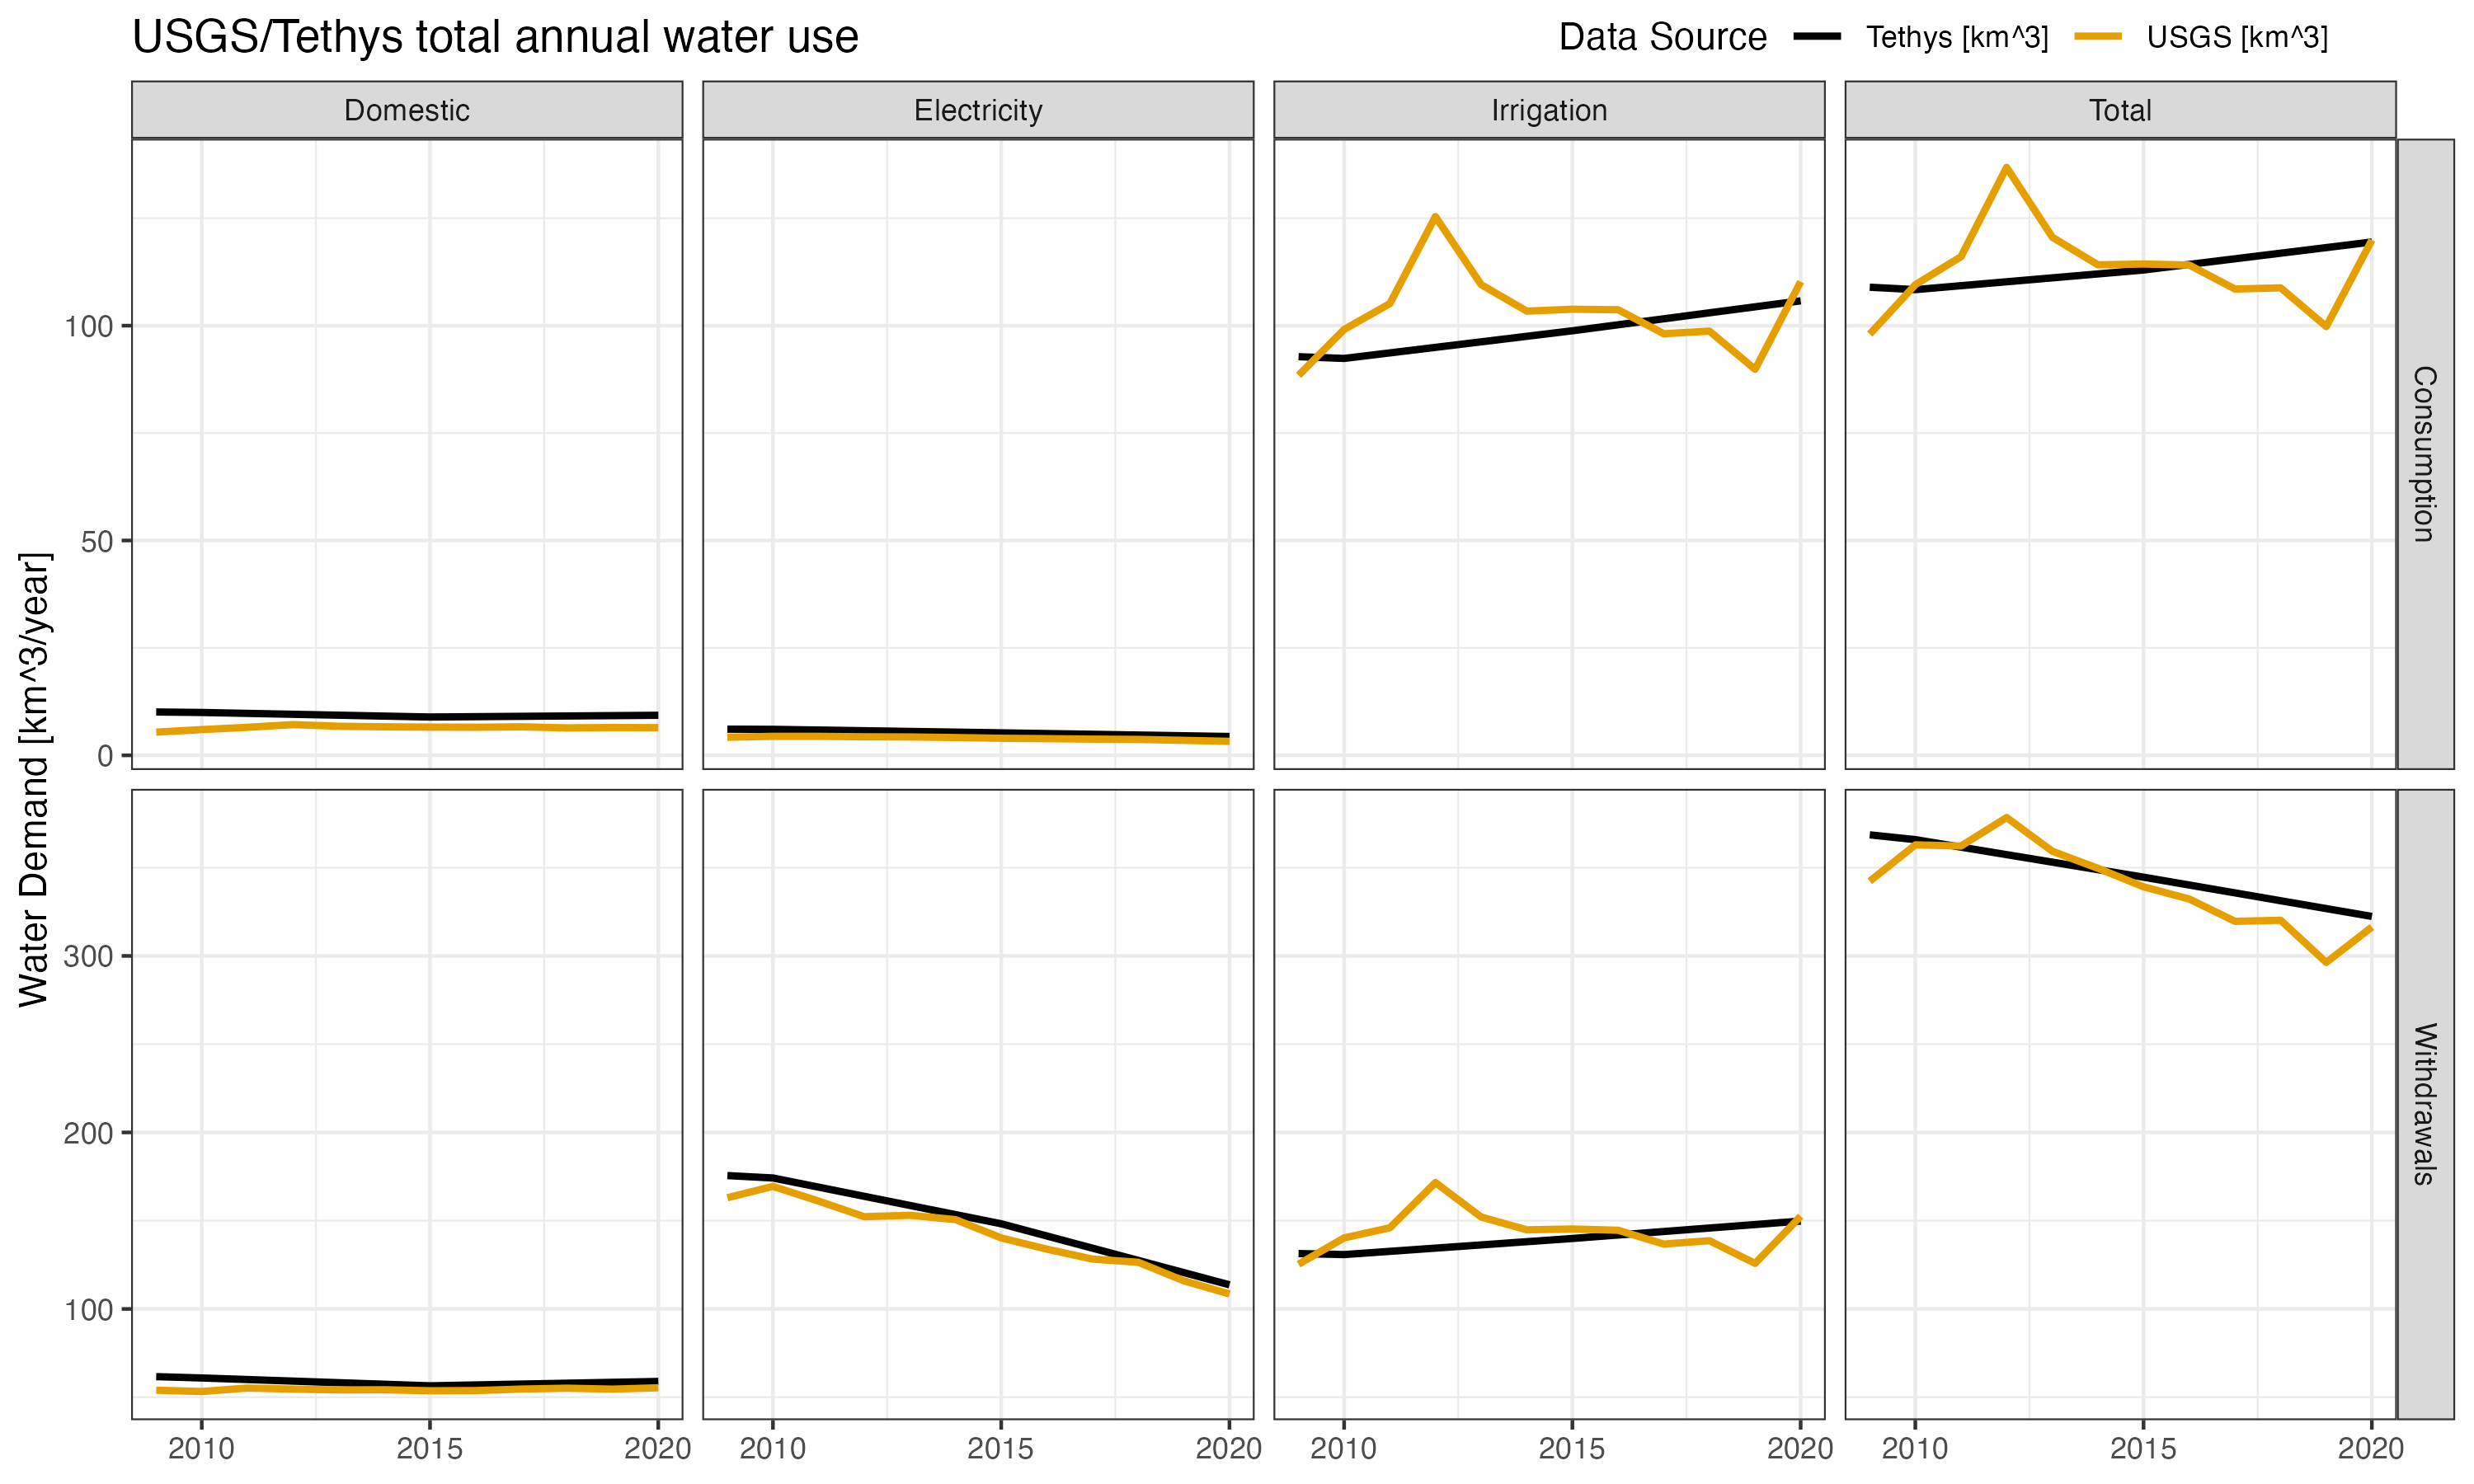
\includegraphics[width=\linewidth]{val1-huc06-usgs-tethys-annual-total.png}
\caption{CONUS annual water use by sector and combined total from Tethys (black solid line) and USGS (orange dashed line) over the harmonized 2010--2019 comparison period (with $1.12\times$ municipal scope adjustment applied to USGS Public Supply in the Domestic and Total panels).}
\label{fig:annual-total-timeseries}
\end{figure}

\begin{figure}[!ht]
\centering
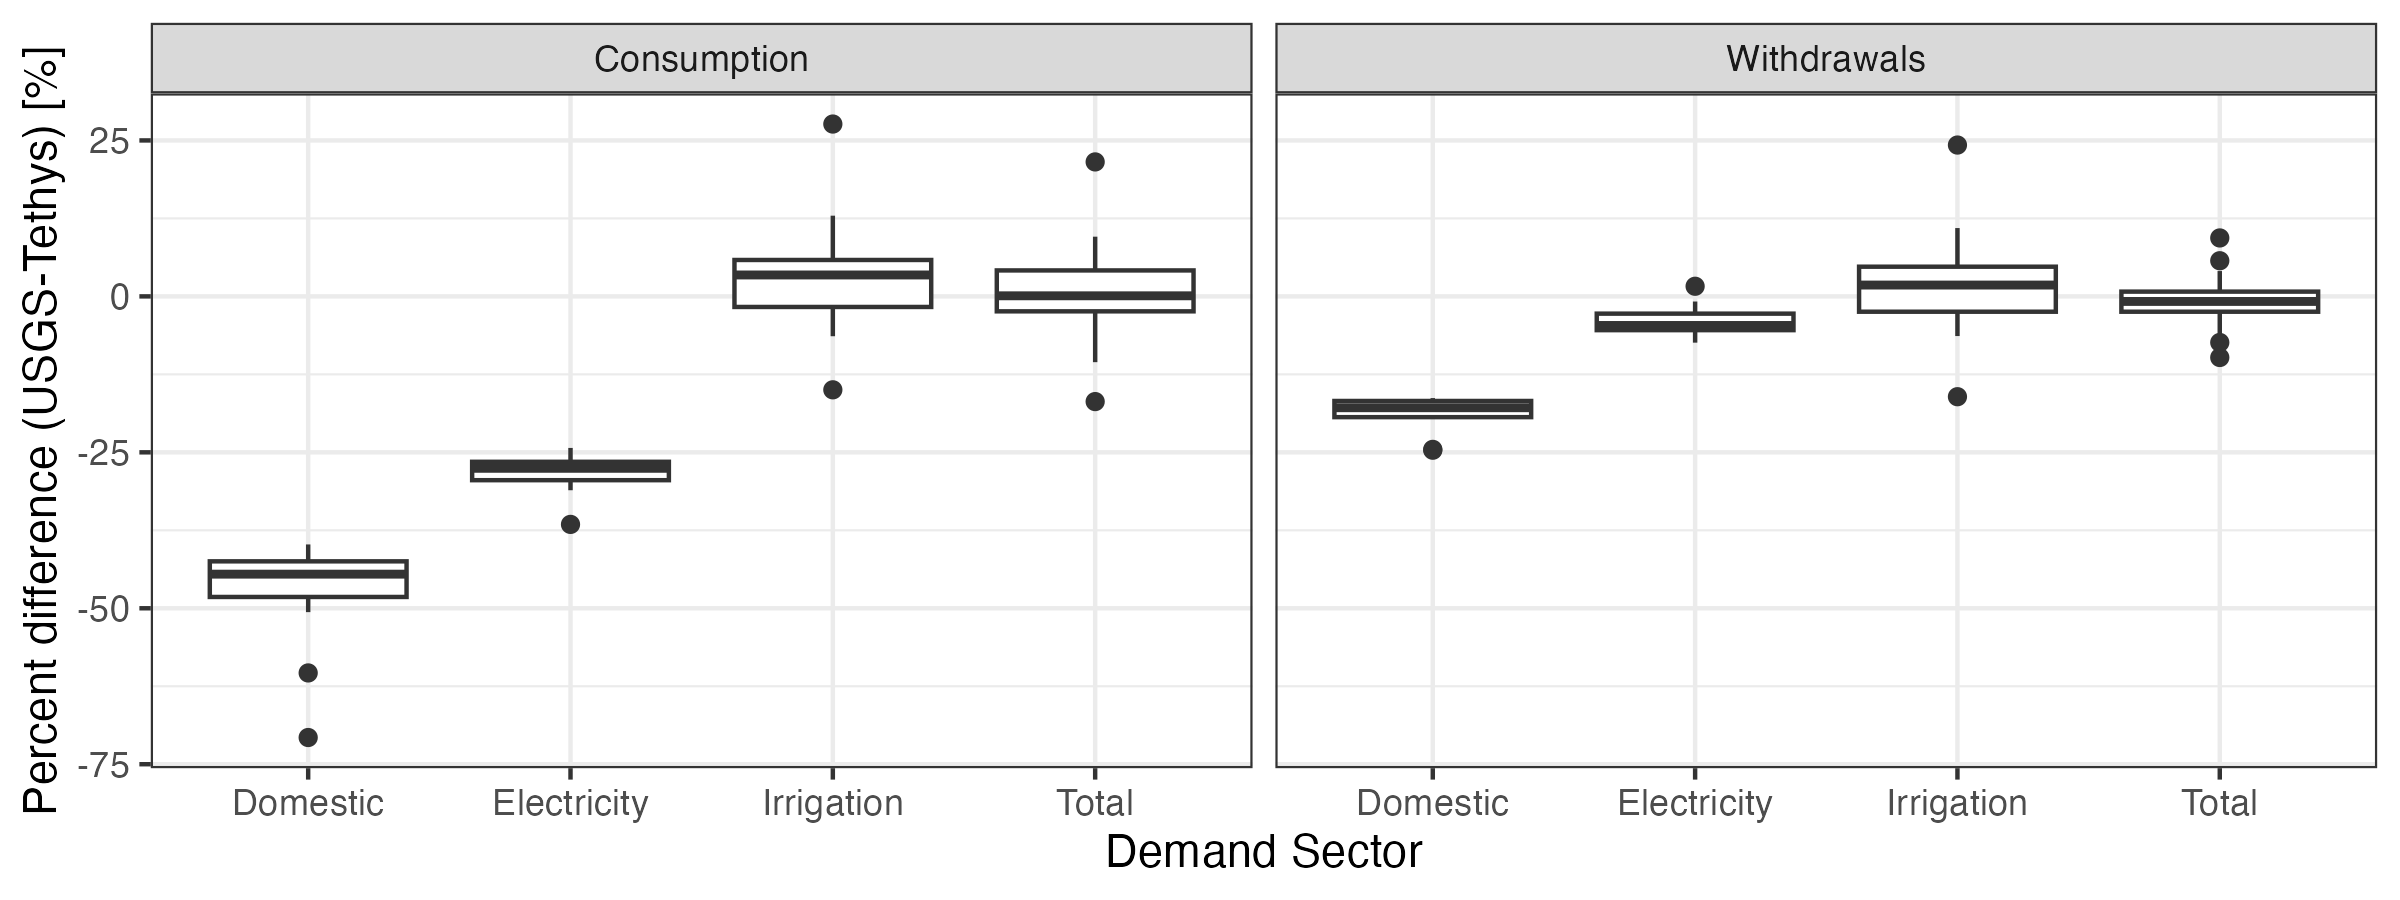
\includegraphics[width=\linewidth]{val2-huc06-usgs-tethys-annual-total-pdiff.png}
\caption{Symmetric percent difference, $100 \times (\text{USGS} - \text{Tethys}) / [(\text{USGS} + \text{Tethys})/2]$, between 2010--2019 mean annual USGS and Tethys water use across HUC6 basins ($n=329$ basins for Domestic and Total, $n=227$ for Electricity withdrawals and $223$ for Electricity consumption, and $n=316$ for Irrigation, excluding basins where USGS reports zero use), by sector and water use type. Boxplot whiskers extend to 1.5 times the interquartile range (IQR), and the dashed line marks zero difference.}
\label{fig:annual-total-boxplot}
\end{figure}

\subsection*{HUC6 spatial agreement}

The symmetric percent difference in 2010--2019 mean annual use at the HUC6 scale is mapped in Figure~\ref{fig:map-pbias}. Each sector's spatial disagreement pattern reflects an identifiable feature of the downscaling chain. Tethys exceeds USGS in the Electricity sector across much of the eastern and interior U.S.: GCAM-USA represents thermoelectric water use at state aggregates that 
% COMMENT-ning: you mean "underestimate"? as lag implies a temporal delay 
lag observed cooling water reductions at individual plants, and the static 2015 GPPD/IM3 plant capacity proxy allocates 
% COMMENT-ning: you mean water demand by fuel type?
fuel demand by installed MW without differentiating plant cooling technologies, contributing to scatter across basins. Tethys and USGS disagree most strongly in western and Plains Irrigation basins, where crop area proxies and distributions weighted by GSI depart from USGS HUC12 estimates under local water management practices. Domestic (municipal) demand tracks USGS Public Supply closely in space ($r=0.95$) while exhibiting a systematic offset linked to scope differences between GCAM-USA municipal demand (which includes self-supplied domestic use) and USGS Public Supply, as well as differences between GCAM-USA base year state calibrations and the 2025 USGS HUC12 reanalysis (whereas the Wada\cite{Wada2011} $R$ parameter in Eq.~\ref{eq:dom-monthly} governs monthly seasonal amplitude rather than annual totals). Basin withdrawal correlations over 2010--2019 (Figure~\ref{fig:huc-correlation}) are strong for annual averages, led by Domestic ($r=0.95$), followed by Irrigation ($r=0.89$) and Electricity ($r=0.72$), with corresponding consumption correlations of $0.71$, $0.91$, and $0.87$. Points in Figure~\ref{fig:huc-correlation} are colored by basin drainage area and show no systematic dependence on basin size.

\begin{figure}[!ht]
\centering
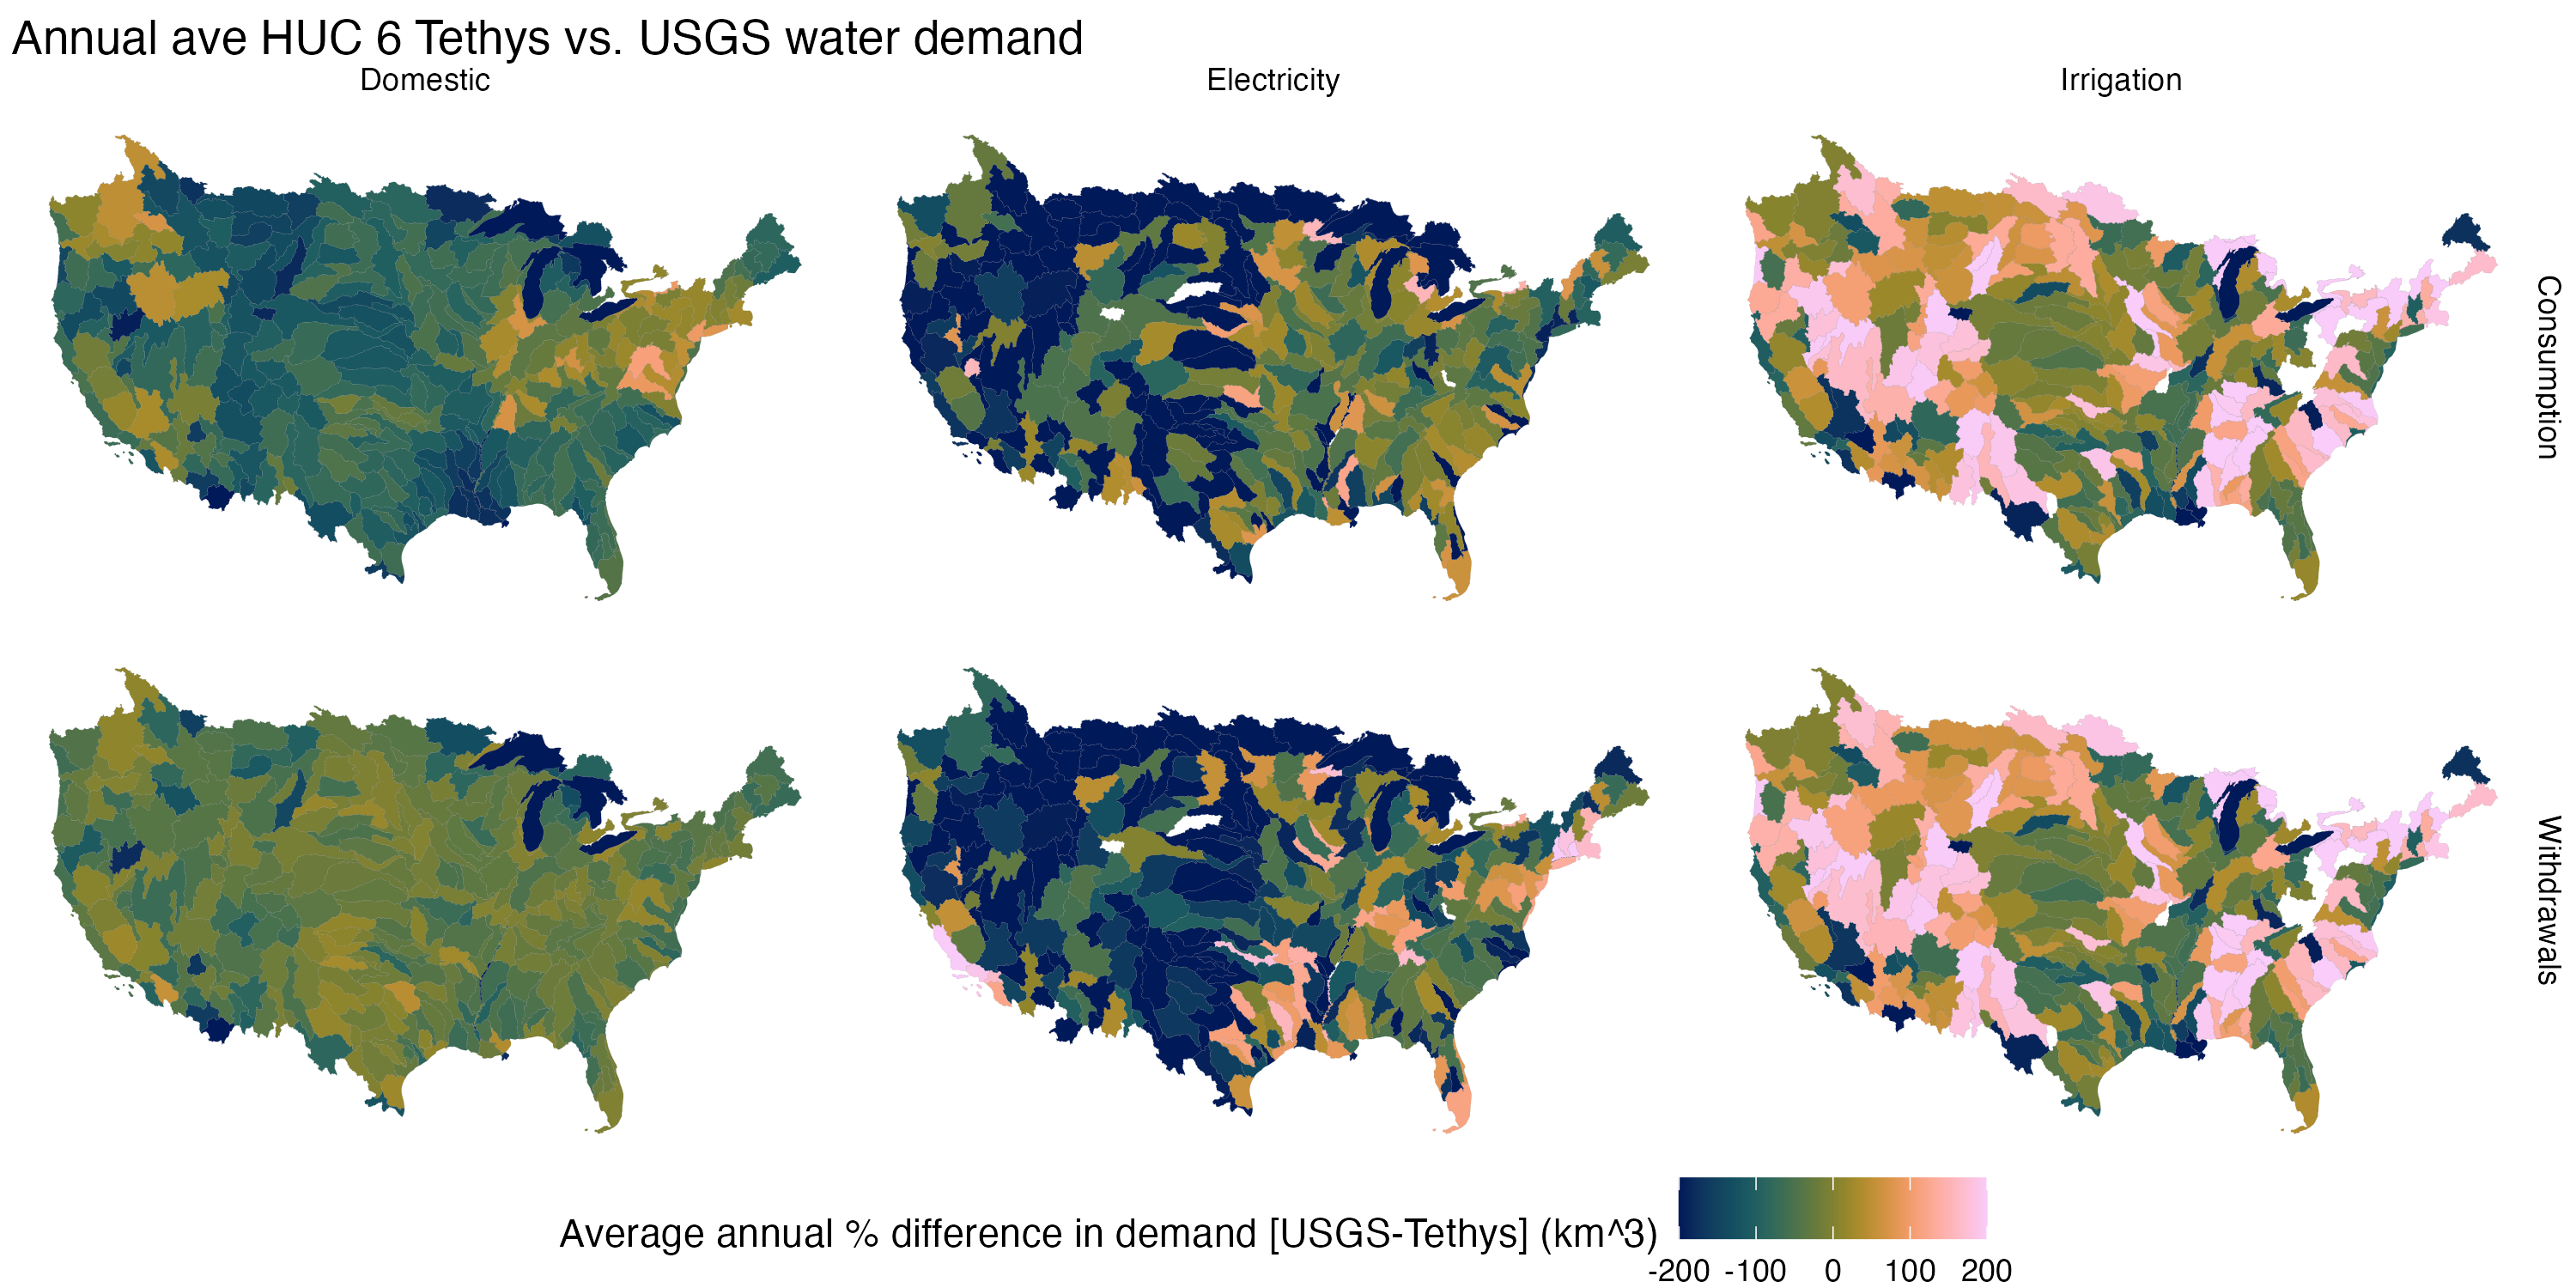
\includegraphics[width=\linewidth]{val3-huc06-pdiff-usgs-tethys.png}
\caption{Symmetric percent difference in mean annual HUC6 water use over 2010--2019, computed as $100 \times (\text{USGS} - \text{Tethys}) / [(\text{USGS} + \text{Tethys})/2]$, for the Domestic (vs.\ $1.12\times$ USGS Public Supply), Electricity, and Irrigation sectors. Colors show USGS minus Tethys: dark blue and green shades indicate Tethys $>$ USGS, and yellow and pink shades indicate USGS $>$ Tethys.}
\label{fig:map-pbias}
\end{figure}

\begin{figure}[!ht]
\centering
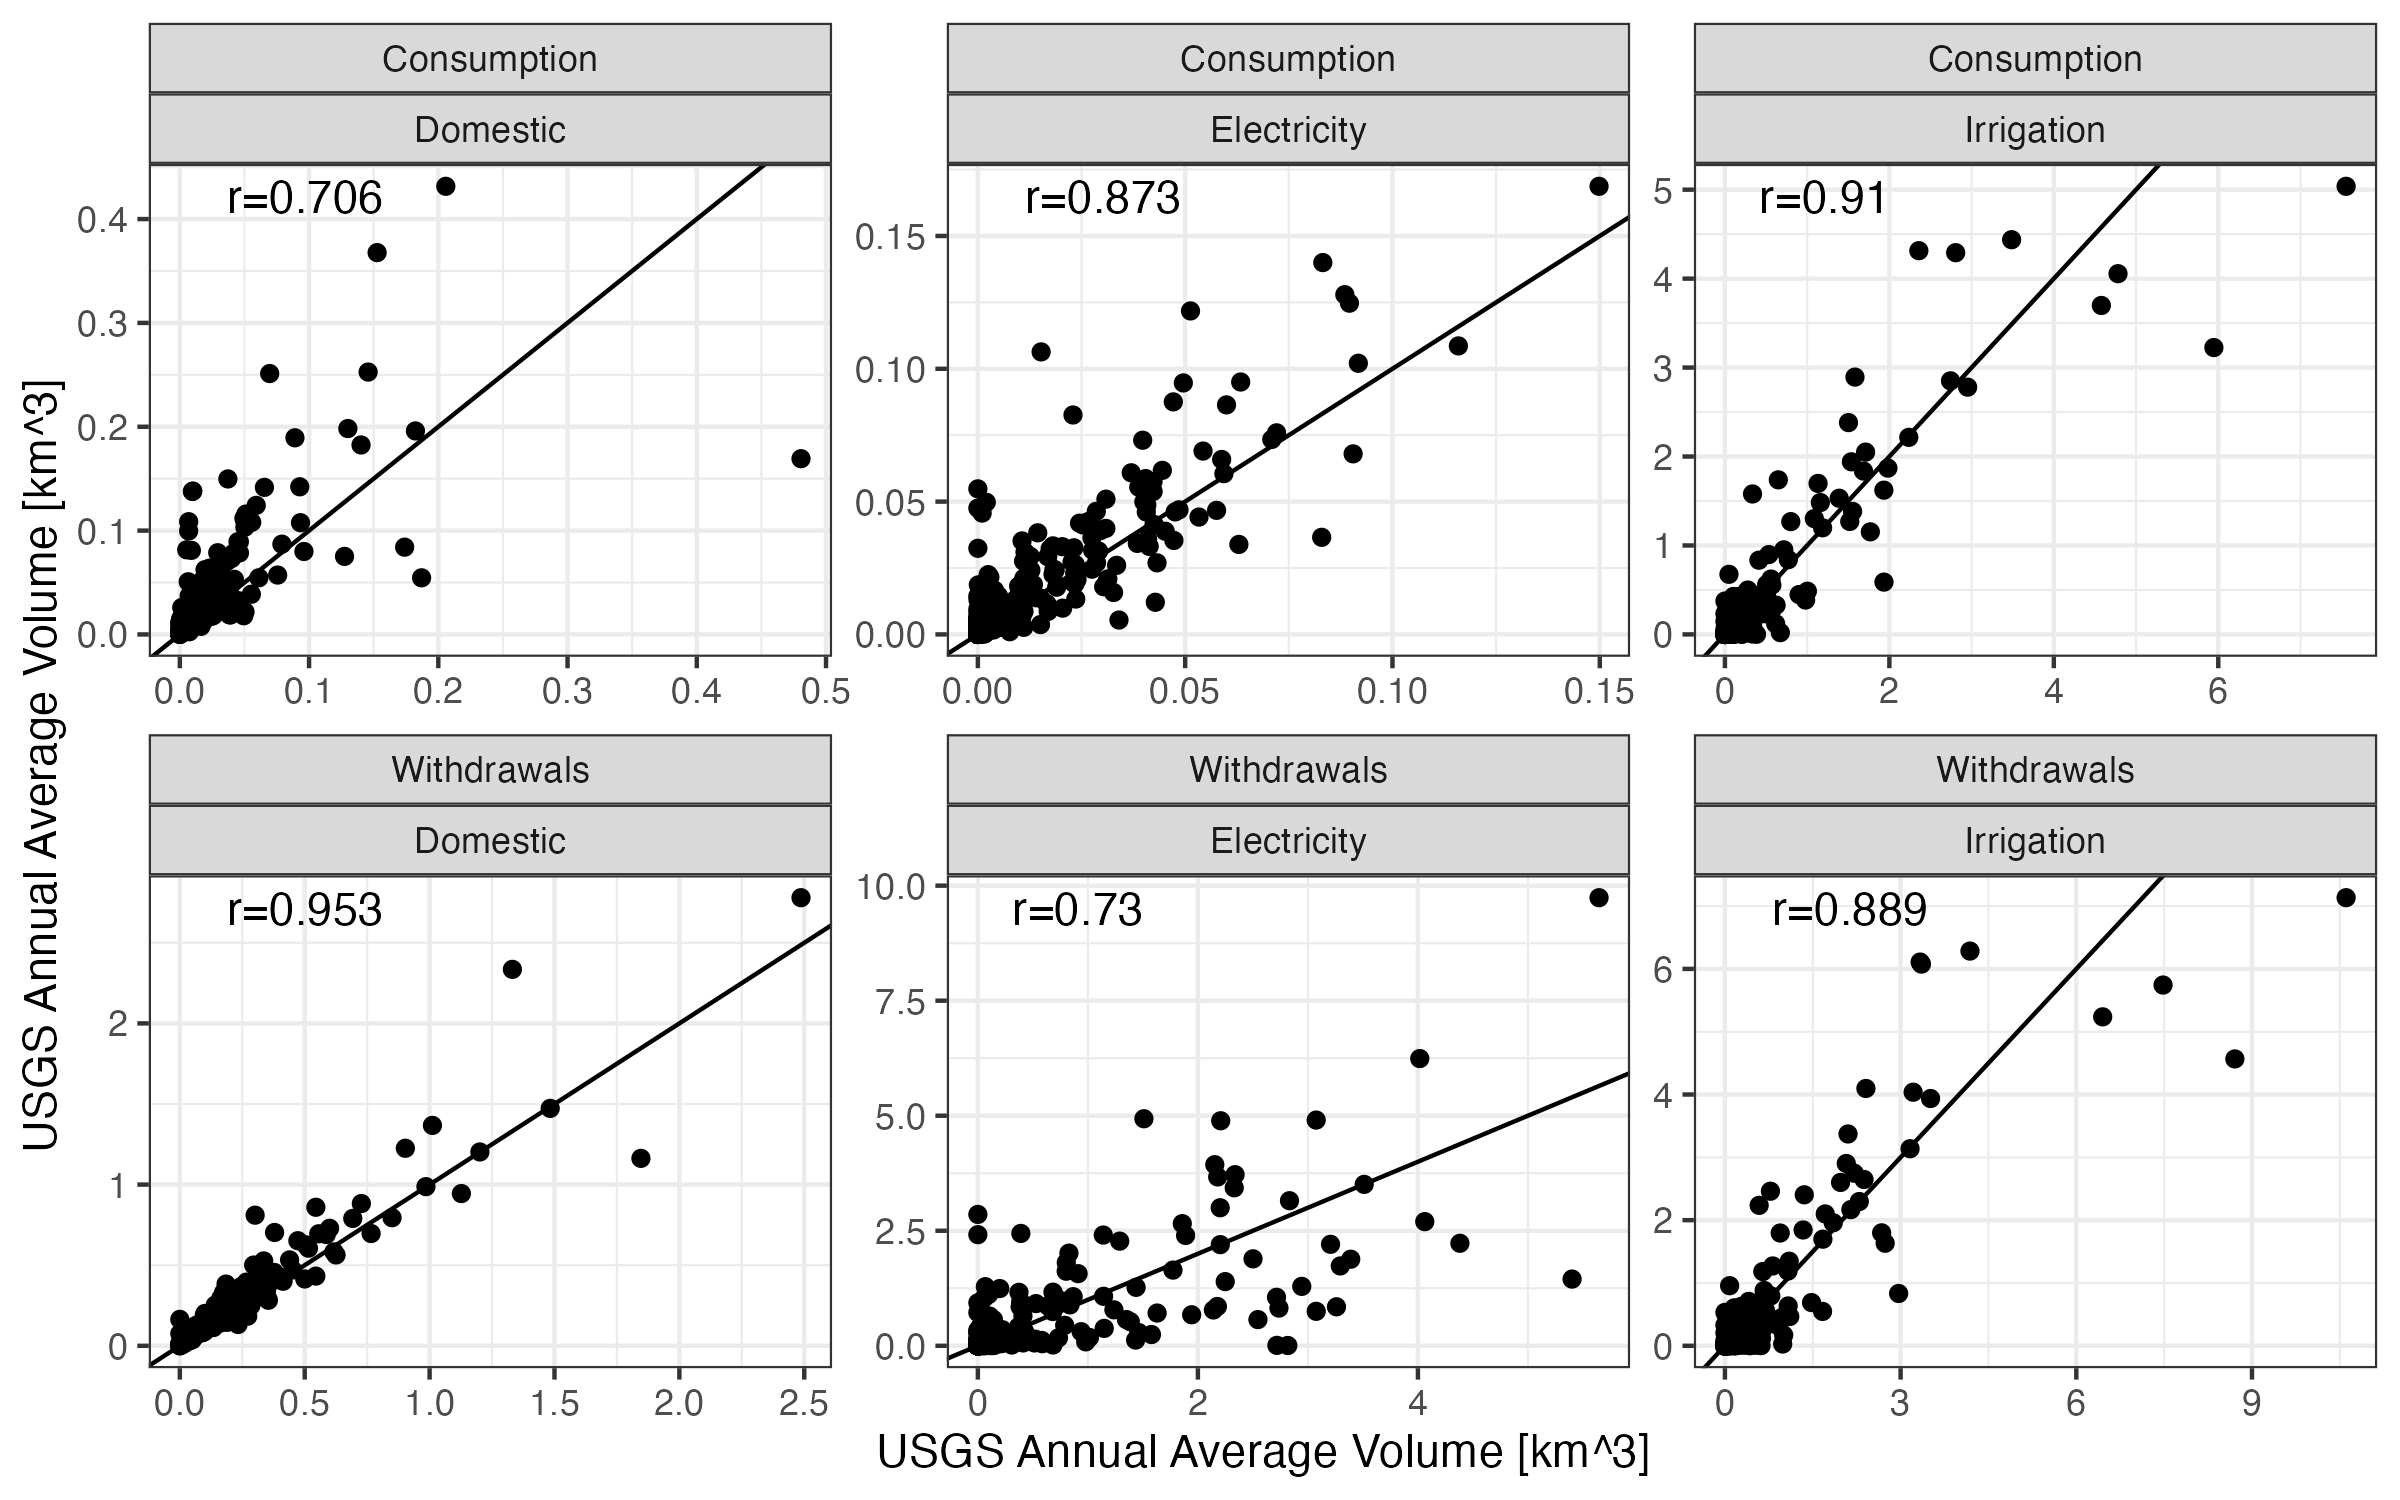
\includegraphics[width=0.92\linewidth]{val4-huc06-scatter-usgs-tethys.png}
\caption{HUC6 mean annual water demand over 2010--2019, Tethys versus USGS, by sector and water use type ($n=329$ basins for Domestic, $227$ for Electricity withdrawals and $223$ for Electricity consumption, and $316$ for Irrigation). Solid lines denote the 1:1 relationship, and points are colored by basin drainage area in km$^2$.}
\label{fig:huc-correlation}
\end{figure}

\subsection*{Seasonal cycle}

Monthly CONUS demands over 2010--2019 are compared in Figure~\ref{fig:monthly}. Irrigation and Domestic withdrawals match the USGS seasonal phase closely, although Tethys Irrigation peaks slightly less sharply in July--August and Domestic reflects the municipal versus public supply level offset. In addition, whereas Eq.~(\ref{eq:dom-monthly}) parameterizes municipal seasonality from temperature alone using a coarse regional amplitude $R$\cite{Wada2011}, USGS Public Supply analyses show that precipitation alongside temperature strongly shapes summer outdoor water use across U.S.\ climate zones\cite{Alzraiee2024WRR,Luukkonen2023USGS,Luukkonen2025JAWRA}. Electricity consumption exhibits a persistent positive offset in months outside summer, reflecting differences in how GCAM-USA and USGS parameterize noncooling and baseload thermoelectric water consumption.

\begin{figure}[!ht]
\centering
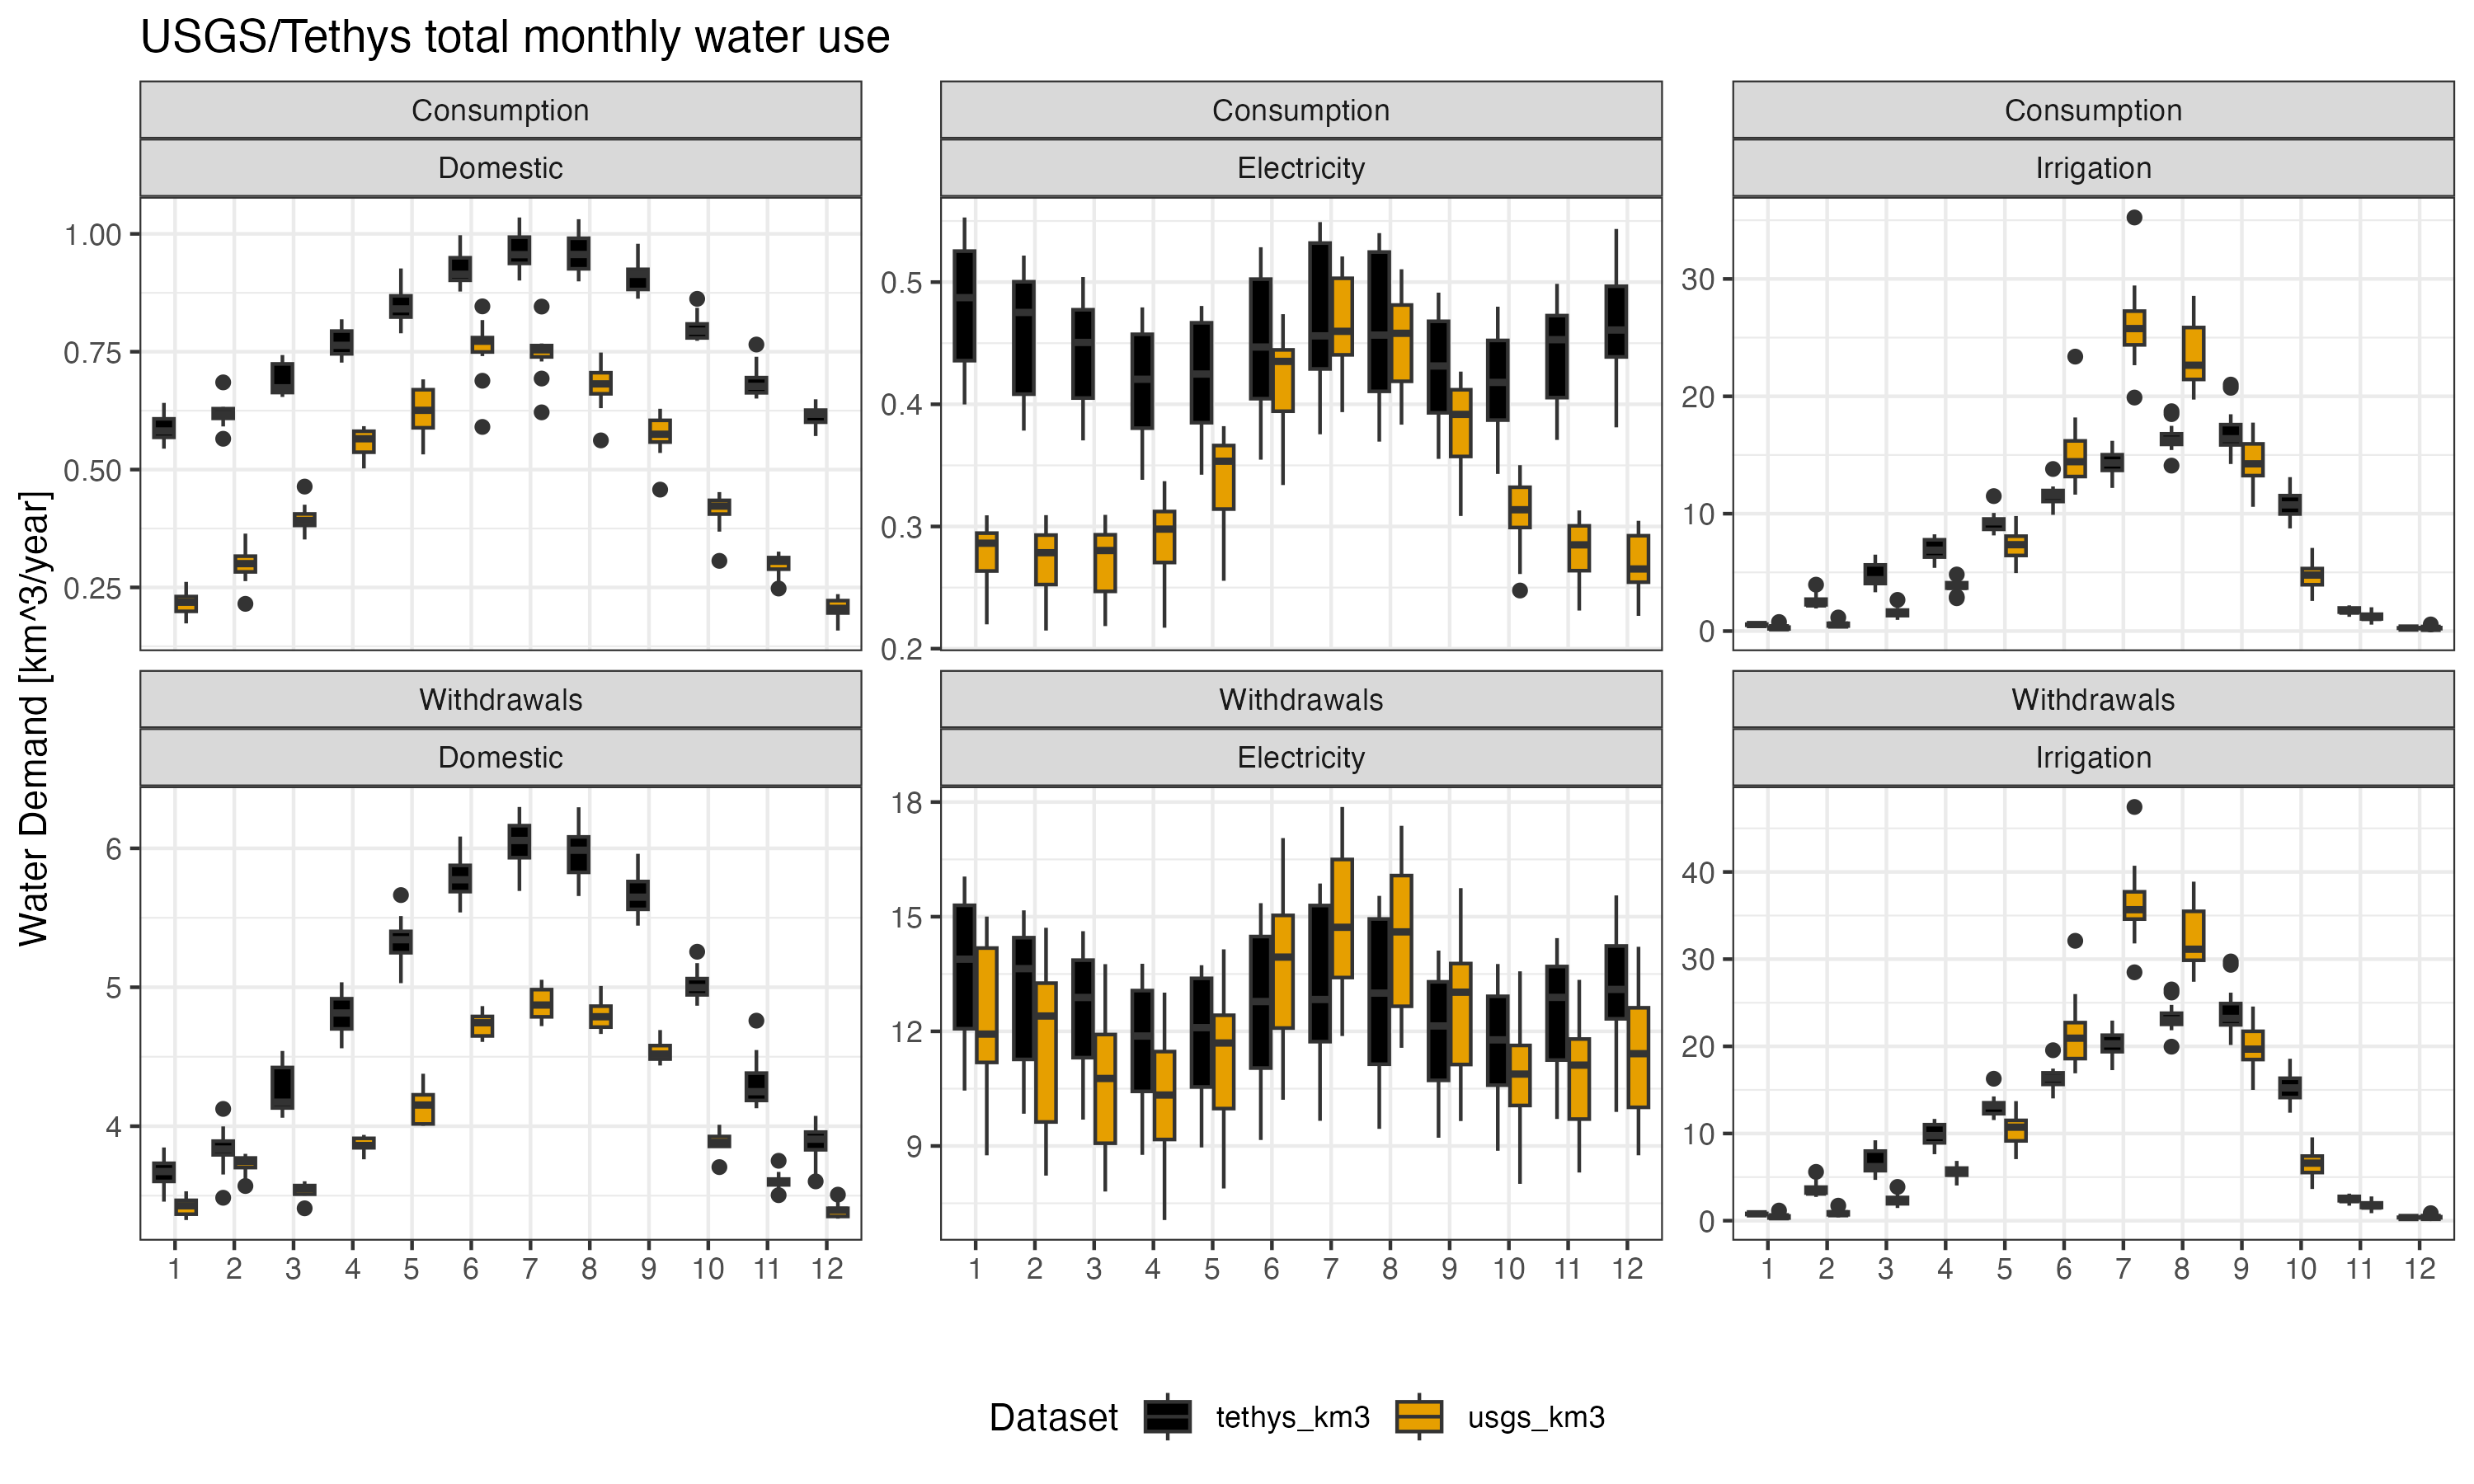
\includegraphics[width=\linewidth]{val5-huc06-usgs-tethys-monthly-total.png}
\caption{Distribution of monthly CONUS water use by sector over 2010--2019 from Tethys (grey) and USGS (orange, with $1.12\times$ scaling applied to Public Supply in the Domestic panels). Boxplot whiskers extend to 1.5 times the IQR across the 10-year comparison window.}
\label{fig:monthly}
\end{figure}

\subsection*{Consistency across scenarios}

CONUS annual withdrawals across the historical baseline and eight future scenarios for the three largest sectors and their sum are shown in Figure~\ref{fig:scenarios} (reported for \texttt{<Sector>\_withdrawals.nc}, excluding irrigation conveyance losses). The step change at 2020 reflects the transition from the ERA5 historical baseline to the TGW future simulations and is a documented feature of the TGW thermodynamic perturbation design\cite{Jones2023TGW} rather than a physical jump. From 2015 historical CONUS withdrawals of $350.3\text{ km}^3\text{ yr}^{-1}$ across all six sectors ($150.7$ Electricity, $116.2$ Irrigation, $56.7$ Domestic, $19.3$ Manufacturing, $4.9$ Mining, and $2.6\text{ km}^3\text{ yr}^{-1}$ Livestock), projected 2100 totals bifurcate sharply by socioeconomic pathway: across the four SSP3 scenarios, CONUS withdrawals decline by $23$--$29\%$ to $249.7$--$268.1\text{ km}^3\text{ yr}^{-1}$, whereas across the four SSP5 scenarios total withdrawals rise by $3$--$22\%$ above 2015 to $359.5$--$428.4\text{ km}^3\text{ yr}^{-1}$.

Distinct sectoral mechanisms govern these trajectories. Electricity withdrawals contract steeply in every future scenario (falling to $8.6$--$20.8\text{ km}^3\text{ yr}^{-1}$ in 2100 under SSP3 and $19.6$--$52.7\text{ km}^3\text{ yr}^{-1}$ under SSP5) as legacy once-through steam plants retire in favor of recirculating cooling and nonthermal renewable generation, reducing surface water withdrawal pressure across eastern river basins. With thermoelectric withdrawals declining, Irrigation becomes the largest withdrawal sector in all eight futures ($178.1$--$199.4\text{ km}^3\text{ yr}^{-1}$ in 2100 under SSP3 and $158.5$--$220.6\text{ km}^3\text{ yr}^{-1}$ under SSP5), with radiative forcing (\texttt{rcp45} versus \texttt{rcp85}) and GCM sensitivity (\texttt{cooler} versus \texttt{hotter}) generating up to $62\text{ km}^3\text{ yr}^{-1}$ of late century spread concentrated in western and Great Plains agricultural basins. Meanwhile, SSP5 population and industrial growth roughly double Domestic ($100.7$--$121.1\text{ km}^3\text{ yr}^{-1}$) and Manufacturing ($48.5$--$53.6\text{ km}^3\text{ yr}^{-1}$) withdrawals by 2100, whereas under SSP3 Domestic declines to $29.4$--$40.4\text{ km}^3\text{ yr}^{-1}$ and Manufacturing to $15.9$--$18.2\text{ km}^3\text{ yr}^{-1}$.

\begin{figure}[!ht]
\centering
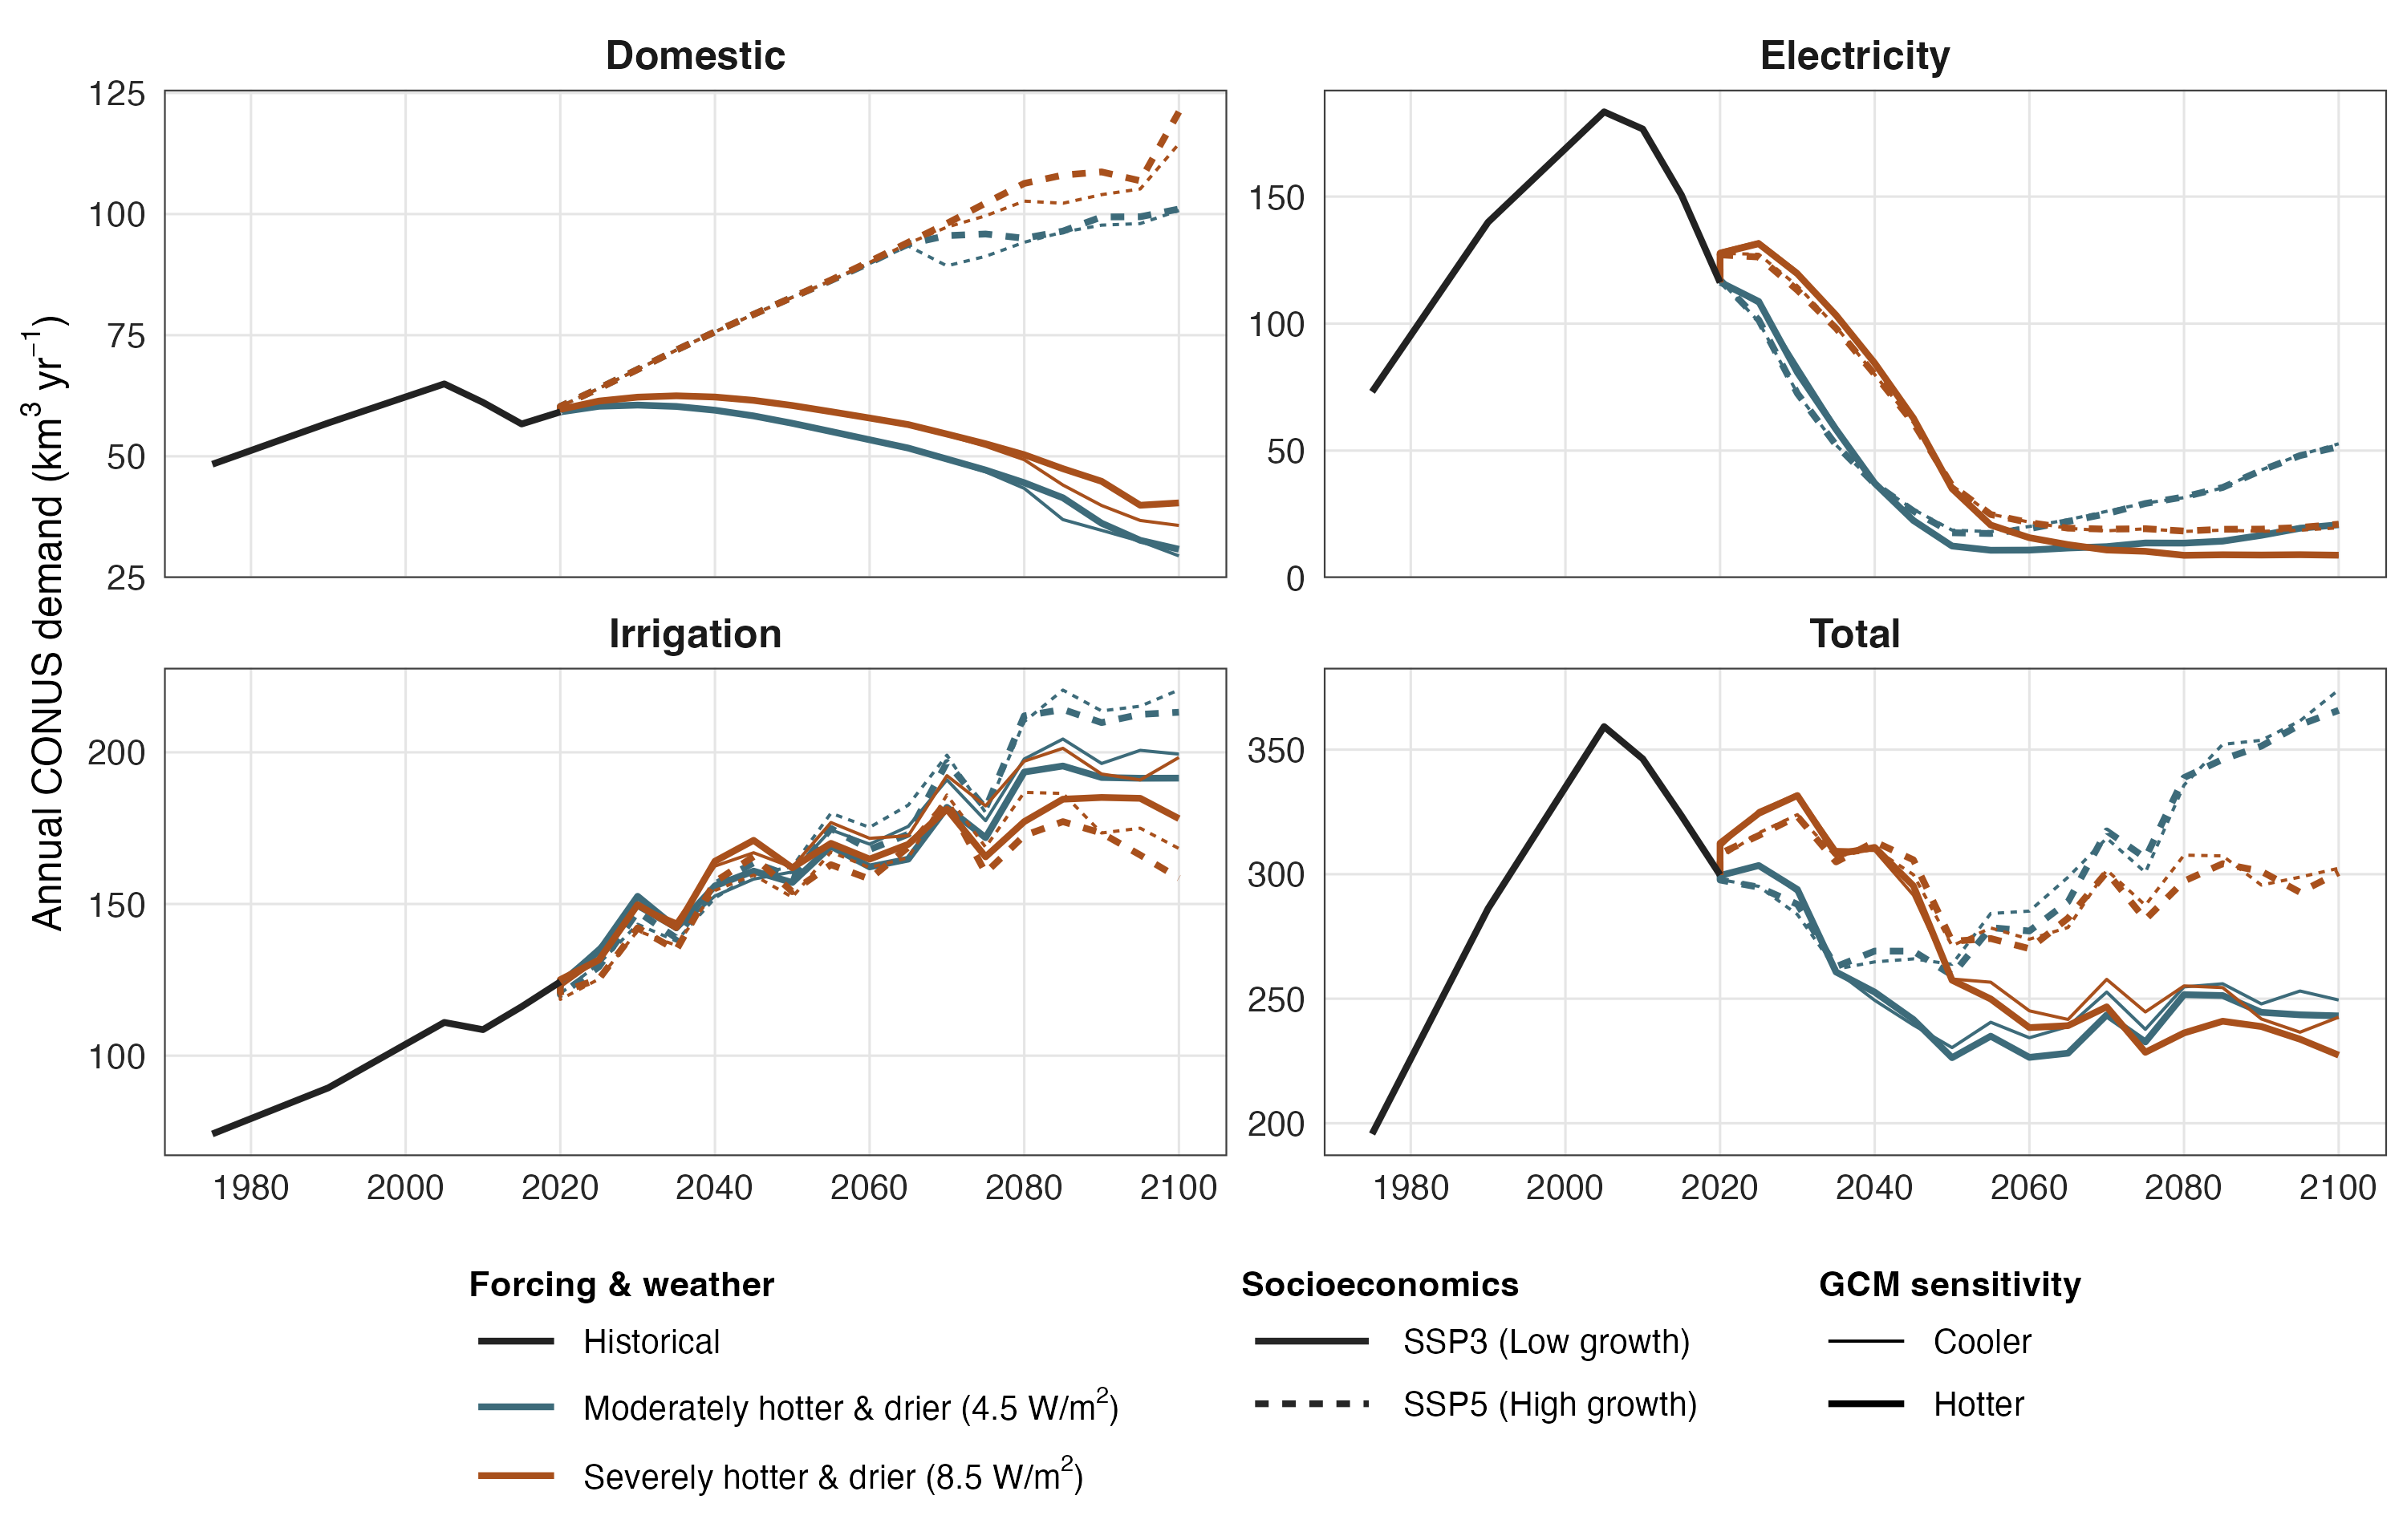
\includegraphics[width=\linewidth]{usage2-projections-annual-conus-timeseries.png}
\caption{Annual CONUS water withdrawals by sector and combined total across historical and future scenarios (excluding irrigation conveyance losses). The historical simulation (black, plotted from the 1975 GCAM-USA anchor through 2020) connects to each of the eight future scenarios in 2020. Future scenarios vary by RCP radiative forcing (color: teal for \texttt{rcp45}, orange for \texttt{rcp85}), SSP socioeconomic pathway (line style: solid for SSP3, dashed for SSP5), and GCM sensitivity group (line width: thin for cooler, thick for hotter). Note that each panel has an independent $y$-axis scale.}
\label{fig:scenarios}
\end{figure}

\subsection*{Sensitivity to downscaling assumptions}

Tethys downscaling conserves regional GCAM-USA demand volumes during spatial allocation (Eq.~\ref{eq:spatial}) and annual volumes for each grid cell during monthly disaggregation (Eqs.~\ref{eq:irr-weights}--\ref{eq:dom-monthly}). To evaluate the sensitivity of the spatial downscaling across all six sectors, we held 2015 regional withdrawals fixed and recomputed HUC6 basin totals under three classes of proxy perturbations (Figure~\ref{fig:sensitivity}a): shifting proxy reference periods, pooling subsector proxies, and substituting empirical 2015 USGS county water use distributions\cite{Dieter2018USGS} or predecessor proxies. Changing the proxy reference periods has minimal impact on basin demand distributions, shifting $1.4\%$ of CONUS \texttt{Domestic} withdrawals across HUC6 basins between 2010 and 2015 SSP population grids (median symmetric absolute percent difference $2.6\%$) and $4.3\%$ of \texttt{Irrigation} withdrawals between 2005 and 2015 Demeter cropland ($12.2\%$). Pooling the 25 GCAM-USA subsectors into single sector proxies has a modest effect in \texttt{Irrigation} ($6.0\%$ HUC6 share shifted, median $20.0\%$) where crop areas overlap within agricultural basins, whereas pooling the seven power plant fuels in \texttt{Electricity} ($22.9\%$ shifted, median $63.6\%$) or replacing the five GLW~3 livestock maps with cattle density alone in \texttt{Livestock} ($33.2\%$ shifted, median $55.7\%$) substantially alters basin totals.

Substituting empirical 2015 USGS county sectoral withdrawals\cite{Dieter2018USGS} as alternative spatial proxies suugests that gridded population and cropland capture substate municipal and agricultural patterns reasonably well ($14.4\%$ and $13.2\%$ of CONUS HUC6 share shifted for \texttt{Domestic} and \texttt{Irrigation}, $r=0.90$ and $0.97$), while GLW~3 aligns moderately with county \texttt{Livestock} ($27.0\%$ shifted, $r=0.70$). Larger structural sensitivities emerge where proxy variables omit specific attributes of water use facilities. In \texttt{Electricity}, replacing plant capacity grouped only by fuel (MW) with county thermoelectric withdrawals reflecting cooling systems shifts $27.2\%$ of HUC6 share (median $90.0\%$), while reverting to the state population proxy used in Tethys~v1\cite{Khan2023} shifts $38.8\%$ of HUC6 share ($94.6\%$ at the 1/8$^{\circ}$ cell scale, $r=0.70$). In the two industrial sectors lacking HUC12 reanalysis benchmarks, replacing state population with USGS county industrial and mining withdrawals reallocates $40.2\%$ of \texttt{Manufacturing} ($r=0.54$, median $81.8\%$) and $51.6\%$ of \texttt{Mining} ($r=0.18$, median $71.4\%$) across HUC6 basins, although their small combined share of 2015 CONUS withdrawals ($6.9\%$) limits the resulting shift in total HUC6 withdrawals across all six sectors to $2.9\%$. Omitting the USGS groundwater and surface water source share adjustment (Eq.~\ref{eq:source-shares}) reduces 2015 CONUS nonelectric groundwater withdrawals from $121.4$ to $40.1\text{ km}^3\text{ yr}^{-1}$ ($-67.0\%$ net volume change and $36.2\%$ HUC6 share reallocated, median $196.3\%$), and including irrigation conveyance losses (\texttt{\_with\_losses}) increases 2015 CONUS irrigation withdrawals by $+20.5\%$ ($140.0$ versus $116.2\text{ km}^3\text{ yr}^{-1}$).

Compared with spatial proxy selection, temporally disaggregated monthly profiles are less sensitive to parameter perturbations than to structural formula choices over 2010--2019 (Figure~\ref{fig:sensitivity}b--d). In \texttt{Irrigation} (Eq.~\ref{eq:irr-weights}, Figure~\ref{fig:sensitivity}b), omitting the moisture deficit term $\Delta_m$ (GSI alone) or reverting to positive temperature weighting ($T_m > 0\,^{\circ}\mathrm{C}$) shifts monthly shares by up to $4.8$ and $4.6$ percentage points relative to the default $\Delta_m \cdot GSI_m$ formulation, flattening warm season peaks away from the sharper July--August USGS profile. In \texttt{Electricity} (Eqs.~\ref{eq:elec-cases}--\ref{eq:elec-demand}, Figure~\ref{fig:sensitivity}c), perturbing the HDD and CDD regime thresholds $(650, 450)$\cite{Huang2018} by $\pm 50\%$ substantially alters CONUS cell and year regime shares ($32\%$ default case~1 versus $49\%$ at $-50\%$ and $20\%$ at $+50\%$) yet changes monthly distributions by at most $0.4$ percentage points ($+1.8$ and $-1.1$ percentage points under unweighted illustrative load shares). Doubling the GCAM-USA cooling load share $p_{\mathrm{cool}}$ lifts July shares by $+1.0$ percentage point toward the USGS summer peak. In \texttt{Domestic} (Eq.~\ref{eq:dom-monthly}, Figure~\ref{fig:sensitivity}d), perturbing Wada's regional amplitude $R$\cite{Wada2011} by $\pm 50\%$ alters any monthly proportion by at most $\pm 1.0$ percentage point around a default profile that matches CONUS USGS Public Supply within a mean absolute error of $0.4$ percentage points. By contrast, a uniform $1/12$ monthly split ($R=0$), as applied to \texttt{Manufacturing}, \texttt{Mining}, and \texttt{Livestock}, dampens summer municipal peaks by $2.0$ percentage points locally, though imposing an illustrative $\pm 30\%$ seasonal cycle on those three minor sectors ($7.6\%$ of CONUS withdrawals combined) alters total CONUS monthly shares across all six sectors by less than $0.2$ percentage points. Overall, projected demand totals are governed primarily by SSP and RCP scenarios (Figure~\ref{fig:scenarios}), watershed patterns by spatial proxy choice and groundwater and surface water source shares (Figure~\ref{fig:sensitivity}a), and monthly timing by meteorological drivers rather than temporal disaggregation parameters (Figure~\ref{fig:sensitivity}b--d).

\begin{figure}[!ht]
\centering
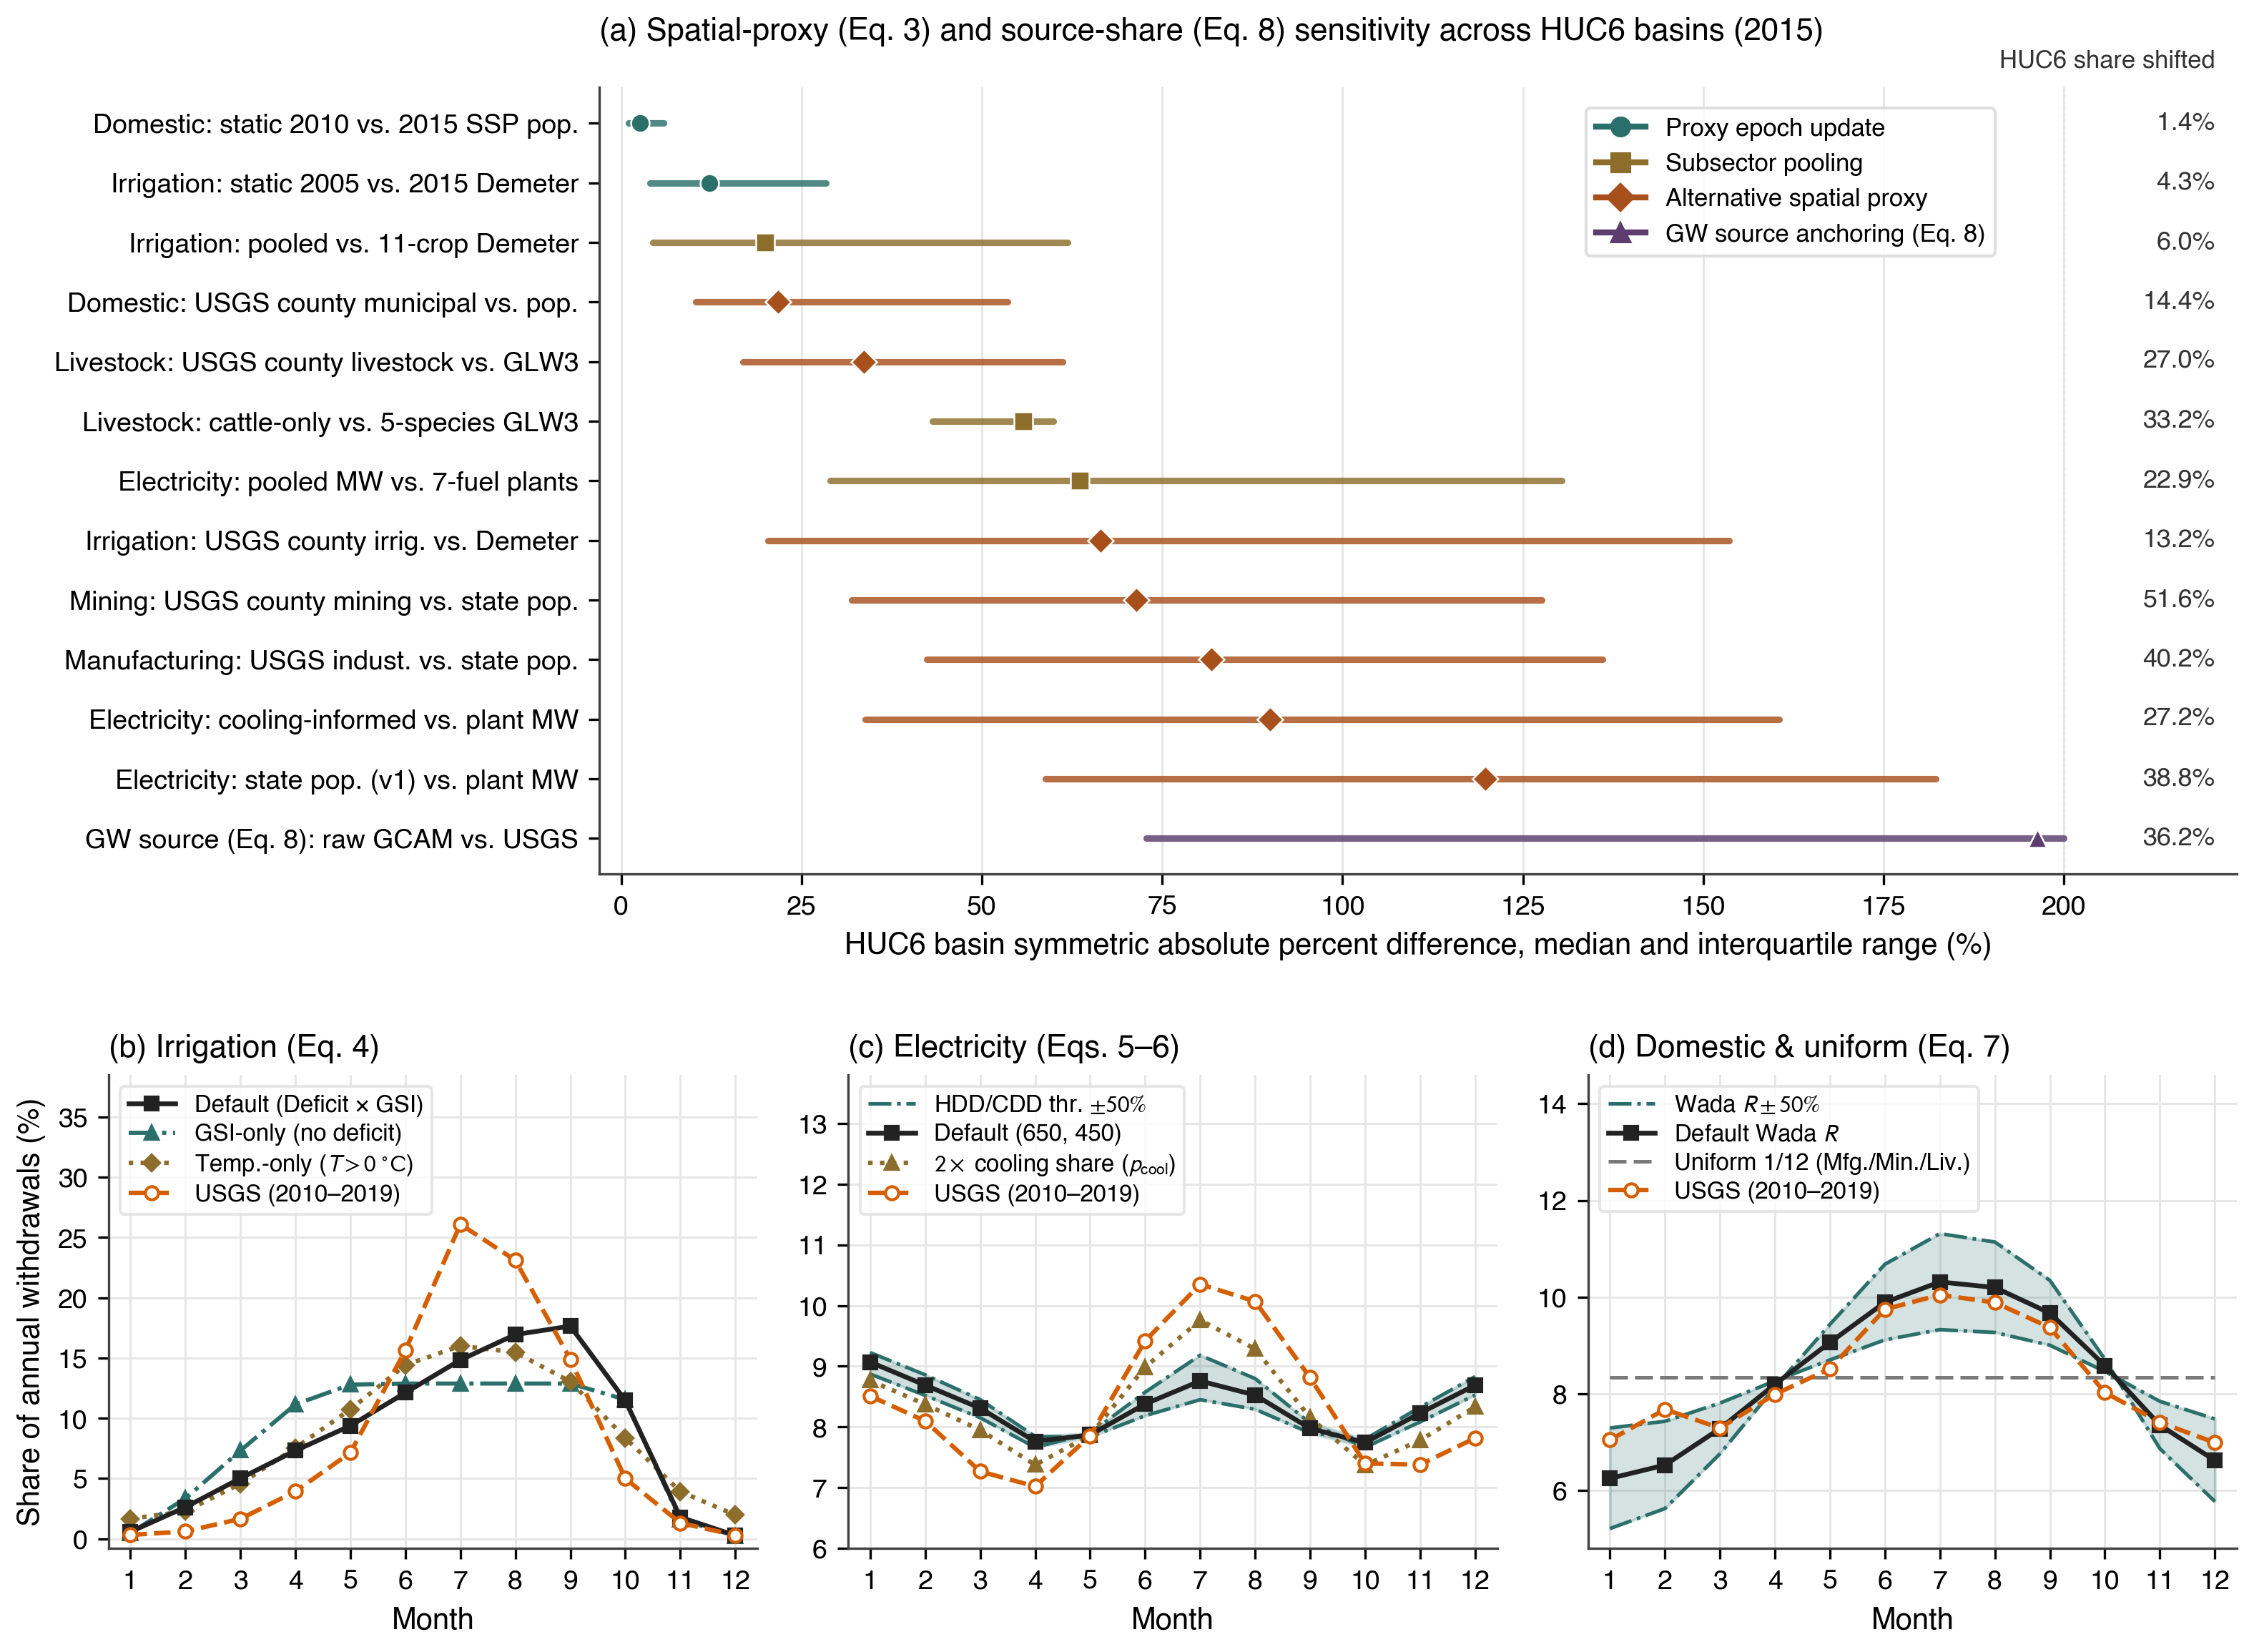
\includegraphics[width=\linewidth]{val6-multisector-sensitivity.png}
\caption{Sensitivity of Tethys water demand estimates across spatial, source share, and temporal downscaling assumptions. (a)~Median and interquartile range of HUC6 symmetric absolute percent differences ($100 \times |\text{Alt} - \text{Base}| / [(\text{Alt} + \text{Base})/2]$) across active CONUS basins in 2015 when holding regional GCAM-USA withdrawals fixed under proxy epoch updates, subsector proxy pooling, alternative empirical county and population proxies\cite{Dieter2018USGS,Khan2023}, and unanchored groundwater source shares versus those anchored to USGS (Eq.~\ref{eq:source-shares}). Values on the right report the percentage of CONUS sectoral volume spatially reallocated across HUC6 basins, measured by total variation distance ($100\% \times \tfrac{1}{2} \sum_b \big|\text{Alt}_b/\!\sum \text{Alt} - \text{Base}_b/\!\sum \text{Base}\big|$, where the $1/2$ factor avoids double counting volume between origin and destination basins). (b--d)~CONUS monthly withdrawal shares weighted by demand over 2010--2019 under parameter and structural perturbations for (b)~\texttt{Irrigation} (Eq.~\ref{eq:irr-weights}), (c)~\texttt{Electricity} (Eqs.~\ref{eq:elec-cases}--\ref{eq:elec-demand}), and (d)~\texttt{Domestic} (Eq.~\ref{eq:dom-monthly}, alongside the uniform $1/12$ profile used for \texttt{Manufacturing}, \texttt{Mining}, and \texttt{Livestock}), benchmarked against 2010--2019 USGS monthly reanalysis profiles.}
\label{fig:sensitivity}
\end{figure}

\subsection*{Limitations}

Several spatial proxy and physical constraint limitations should guide downstream use of the dataset. First, the GLW~3 livestock headcount map\cite{Gilbert2018} is held fixed at its 2010 reference year across all scenarios. Although livestock accounts for $\approx$1--2\% of CONUS water demand, static spatial weights miss regional herd shifts. Newer FAO GLW~4 grids (2015 and 2020 reference years) can update contemporary baselines in future releases, though combining GLW versions across reference years requires harmonizing underlying subnational census predictors to avoid methodological artifacts. Second, state population serves as the spatial proxy for manufacturing and mining, which misses localized industrial or extraction facilities and produces the rural eastern state border transitions seen in Figure~\ref{fig:dominant-sector}. Incorporating county sectoral gross domestic product (GDP) or facility permit registries offers a direct path to refine industrial allocation. Third, while GCAM-USA and CERF model cooling technologies, the Tethys capacity proxy aggregates thermoelectric plants into seven fuel subsectors without cooling system differentiation, which can overallocate withdrawals to recirculating plants and underallocate withdrawals to once-through plants of the same fuel within a state\cite{Peer2016ERL,Sjostedt2025EST}. Fourth, although GCAM-USA constrains basinwide nonrenewable groundwater extraction through depletion supply cost curves\cite{Binsted_2022,Niazi2024PeakWater}, Tethys does not enforce grid cell physical aquifer storage caps at 1/8$^{\circ}$. In subregions experiencing acute depletion such as the southern High Plains Aquifer\cite{Steward2016AWM} and alluvial basins of the Lower Colorado River Basin\cite{Abdelmohsen2025GRL}, late-century groundwater demand projections represent potential demand conditional on basin economics and may exceed locally extractable storage.

Four additional limitations concern temporal downscaling and conveyance losses. First, the simplified GSI in Eqs.~(\ref{eq:gsi-components})--(\ref{eq:gsi-monthly}) omits the vapor pressure deficit (VPD) term of Jolly et al.\cite{Jolly_2005} following Moore et al.\cite{Moore_2015}, which may underweight drought months in humid regions where VPD limits stomatal conductance. Second, Eq.~(\ref{eq:dom-monthly}) drives municipal seasonality from temperature alone\cite{Wada2011} without precipitation controls on outdoor landscape irrigation\cite{Luukkonen2023USGS,Luukkonen2025JAWRA}, while livestock, manufacturing, and mining use a uniform $1/12$ monthly split that understates summer demand peaks in cells where grazing, dairy, industrial cooling, or warm season mining dominate locally\cite{Hou2024ESSD,Grogan2022GMD,LeRiche2017Water}. Third, irrigation files are released both with and without conveyance losses (\texttt{\_with\_losses} suffix), so users coupling to hydrologic models should select the variant matching their routing loss formulation. Fourth, linear interpolation of 5-year GCAM-USA outputs smooths annual drought anomalies relative to observed interannual variability.

% -----------------------------------------------------------------------------
\section*{Usage Notes}

This dataset provides a high-resolution spatiotemporal representation of water demand and source dependence, enabling coupling of sectoral water use with RCP/SSP scenarios, hydrologic, energy, agricultural, and socioeconomic models across historical and future periods through the end of the 21st century. Curated modeling roles and representative applications are summarized in Table~\ref{tab:water_demand_roles}. Beyond traditional hydrologic and integrated assessment modeling, the gridded thermoelectric withdrawal and consumption fields can provide baseline cooling water context for emerging electricity load studies, including regional water resource assessments around hyperscale data centers and artificial intelligence (AI) compute expansion, as well as evaluations of state and local water management policies. When evaluating local scarcity or long-term groundwater sustainability in heavily pumped aquifers, users should consult the basin validation metrics (Table~\ref{tab:validation-metrics}, Figure~\ref{fig:map-pbias}) and couple the gridded demands and groundwater and surface water source shares with physically based groundwater or conjunctive use models (Table~\ref{tab:water_demand_roles}).

\begin{table}[!ht]
\centering
\small
\begin{tabular}{p{3.2cm} p{4.5cm} p{8.4cm}}
\hline
\textbf{Role} & \textbf{Description} & \textbf{Mechanism / Model Integration Use Cases} \\
\hline

Hydrologic and Earth System Model Forcing Variables &
Input to hydrologic, groundwater, and Earth system models as anthropogenic water demand across sectors &
Exogenous water use input as a demand component in water balance and scarcity calculations (e.g., demand/renewable supply), or as a model input in river routing, groundwater, or land surface models such as MOSART-WM\cite{hess-17-4555-2013}, MODFLOW\cite{modflow6}, Superwell\cite{superwell}, ParFlow\cite{parflow}, VIC\cite{vic}, CLM\cite{clm5}, PCR-GLOBWB\cite{pcrglobwb}, and CWatM\cite{cwatm}. \\

Integrated Water Use Scenario Drivers &
Integrates future SSP and RCP pathways and connects water, energy, agriculture, land, and climate systems &
Future demand trajectories in integrated assessment models or regional impacts and adaptation studies as an information exchange mechanism linking hydrology, energy, and crop models, e.g., GCAM\cite{Calvin2019GCAM}, MESSAGEix\cite{messageix}, GLOBIOM\cite{globiom}, and CLIMADA\cite{climada}. \\

Decision Support &
Supports planning, policy, resource management, and human decision making &
Input to optimization, reservoir operations, agent-based, state and local water policy evaluation, and electricity and data center siting and drought planning models for infrastructure investment and water allocation planning, e.g., GEB\cite{geb} and CERF\cite{Vernon2021}. \\

Machine Learning Feature Dataset &
Predictor variable for statistical and machine learning models &
Feature set for Random Forest, XGBoost, LSTM, GNN, and other predictive models for drought impacts, crop yields, groundwater depletion, water scarcity, and infrastructure risk. \\

\hline
\end{tabular}
\caption{Roles of the Tethys gridded water demand dataset with representative model integrations and potential use cases for modeling communities and decision makers.}
\label{tab:water_demand_roles}
\end{table}

We distribute the dataset as NetCDF-4 files containing \texttt{year} and (for monthly files) \texttt{month} dimensions. Each file reports either withdrawals or consumption in km$^3$~yr$^{-1}$ (annual files) or km$^3$~month$^{-1}$ (monthly files) as documented in file metadata. Users may convert annual rates from km$^3$~yr$^{-1}$ to million gallons per day (MGD) by multiplying by $264{,}172.05124/365$, so $1\text{ km}^3\text{ yr}^{-1} \approx 723.76$~MGD.

The integration metarepository\cite{cambrackenIMMMSFATethys_integration_metarepoV1012026} (see Code availability) provides spatial aggregation utilities to map the 1/8$^{\circ}$ grid onto HUC2, HUC4, HUC6, HUC8, or HUC12 watershed polygons; see the metarepository README for usage examples.

% -----------------------------------------------------------------------------
\section*{Data availability}

The Tethys 1/8$^{\circ}$ monthly CONUS sectoral water demand dataset described in this paper, including the YAML run configurations for each scenario, is openly available under a Creative Commons Attribution 4.0 International (CC~BY~4.0) license on MSD-Live (\url{https://doi.org/10.57931/3366643}). Preprocessed model input datasets and region masks needed to reproduce the workflow are openly archived under CC~BY~4.0 in the companion input dataset on MSD-Live (\url{https://doi.org/10.57931/3366010}). Third-party input and validation datasets are publicly available from their respective repositories: GCAM-USA IM3 Phase~2 simulation outputs on MSD-Live (\url{https://doi.org/10.57931/2428940}), TGW meteorological forcing on MSD-Live (\url{https://tgw-data.msdlive.org/}), NASA SEDAC 1/8$^{\circ}$ global SSP population grids (\url{https://doi.org/10.7927/m30p-j498}) and Zenodo U.S.\ state SSP population projections (\url{https://doi.org/10.5281/zenodo.3756179}), Gridded Livestock of the World v3 (GLW~3) on Harvard Dataverse (\url{https://doi.org/10.1038/sdata.2018.227}, \url{https://dataverse.harvard.edu/dataverse/glw_3}), the World Resources Institute Global Power Plant Database v1.3 (\url{https://datasets.wri.org/dataset/globalpowerplantdatabase}), and the USGS HUC12 water use reanalysis data releases for crop irrigation (\url{https://doi.org/10.5066/P9LGISUM}), thermoelectric power (\url{https://doi.org/10.5066/P9ZE2FVM}), and public supply (\url{https://doi.org/10.5066/P9FUL880}), synthesized in Medalie et al.\ (2025, \url{https://doi.org/10.3133/pp1894D}) and distributed via the USGS National Water Availability Assessment Data Companion (\url{https://water.usgs.gov/nwaa-data/}).

\section*{Code availability}

The Tethys spatiotemporal downscaling package\cite{niazi_2026_20552731} (v2.2, BSD 2-Clause license) is openly available on GitHub (\url{https://github.com/JGCRI/tethys}) and archived on Zenodo (\url{https://doi.org/10.5281/zenodo.1300872}). The integration metarepository\cite{cambrackenIMMMSFATethys_integration_metarepoV1012026} (\texttt{tethys\_integration\_metarepo} v1.0.1, CC~BY~4.0 license) containing all preprocessing, scenario execution, workflow configurations, groundwater and surface water postprocessing, HUC aggregation, and validation and figure scripts is openly available on GitHub (\url{https://github.com/IMMM-SFA/tethys_integration_metarepo}) and archived on Zenodo (\url{https://doi.org/10.5281/zenodo.20600510}). Upstream open-source spatial proxy models are available on GitHub for Demeter\cite{Vernon-2018} (\url{https://github.com/IMMM-SFA/demeter}) and CERF\cite{Vernon2021} (\url{https://github.com/IMMM-SFA/cerf}).

% -----------------------------------------------------------------------------
\section*{Acknowledgments}

This research was supported by the U.S.~Department of Energy, Office of Science, as part of research in the Earth and Environmental System Modeling Program. We thank the TGW team for the downscaled climate product, the GCAM-USA team for the scenario simulations, and the USGS water use program for the datasets used for evaluation in this paper.

\section*{Author contributions statement}

C.B.~coordinated the downscaling runs, conducted the HUC comparison against USGS data, developed the sensitivity analysis, packaged the dataset, and drafted this version of the manuscript based on an earlier draft by I.T. 
H.N.~developed and maintained the Tethys model, conducted the runs, and helped with the interpretation of GCAM-USA and Tethys outputs. 
T.T.~extended the Tethys package to support GCAM-USA inputs, developed the first version of the Tethys metarepository, and carried out the initial scenario runs. 
I.T.~wrote the initial draft of this manuscript and contributed to the CERF and Tethys integration and power plant proxy construction. 
K.T.~developed the groundwater and surface water source share postprocessing framework anchored to USGS for Tethys and conducted the associated runs and analyses. 
H.E.~produced the TGW preprocessing pipeline for PET, HDD/CDD, and GSI. 
K.M.~developed the CERF and Tethys integration and power plant proxy construction. 
N.V.~contributed to scenario design and interpretation. 
N.S.~contributed to scientific review, scenario design, and interpretation. 
J.R.~provided overall project guidance and scientific review. 

\section*{Competing interests}

The authors declare no competing interests.

\bibliography{bib/Tethys}

\end{document}
